% !TEX program = xelatex
% !BIB program = bibtex
\documentclass[UTF8,a4paper,12pt,zihao=-4]{ctexart}

% 页面与版式
\usepackage[top=2.5cm,bottom=2.5cm,left=2.6cm,right=2.6cm,headheight=15pt]{geometry}
\usepackage{setspace}
\onehalfspacing
\usepackage{fancyhdr}
\usepackage{lastpage}

% 数学与符号
\usepackage{amsmath,amssymb,amsfonts,mathtools}
\usepackage{bm}
\usepackage{siunitx}

% 图表与浮动体
\usepackage{graphicx}
\usepackage{booktabs}
\usepackage{longtable}
\usepackage{multirow}
\usepackage{array}
\usepackage{float}
\usepackage{caption}
\usepackage{subcaption}
\captionsetup{font=small,labelfont=bf,labelsep=space}

% 绘图
\usepackage{tikz}
\usetikzlibrary{shapes.geometric,arrows.meta,positioning,fit,calc,backgrounds}

% 代码列表与颜色
\usepackage{xcolor}
\usepackage{listings}
\usepackage{enumitem}

% 东南大学毕业论文要求的 GB/T 7714 顺序编码制参考文献
\usepackage[sort&compress]{gbt7714}

% 超链接（置于导言区末尾）
\usepackage[colorlinks=true,linkcolor=black,citecolor=blue!70!black,urlcolor=blue!70!black]{hyperref}

% 待填占位符宏
\newcommand{\todo}[1]{\textcolor{red!80!black}{\textbf{[待填 #1]}}}

% 常用数学算子
\DeclareMathOperator*{\argmin}{arg\,min}
\DeclareMathOperator{\diag}{diag}
\DeclareMathOperator{\clip}{clip}
\DeclareMathOperator{\wrap}{wrap}
\newcommand{\SE}{\mathrm{SE}(3)}
\newcommand{\SO}{\mathrm{SO}(3)}
\newcommand{\so}{\mathfrak{so}(3)}

% 代码排版样式
\definecolor{codebg}{RGB}{248,249,250}
\definecolor{codeframe}{RGB}{218,222,228}
\definecolor{codekw}{RGB}{0,92,197}
\definecolor{codecm}{RGB}{106,115,125}
\definecolor{codestr}{RGB}{3,47,98}

\lstset{
  language=Python,
  basicstyle=\footnotesize\ttfamily,
  backgroundcolor=\color{codebg},
  frame=single,
  rulecolor=\color{codeframe},
  keywordstyle=\color{codekw}\bfseries,
  commentstyle=\color{codecm}\itshape,
  stringstyle=\color{codestr},
  numbers=left,
  numberstyle=\tiny\color{gray},
  numbersep=8pt,
  breaklines=true,
  showstringspaces=false,
  tabsize=4,
  xleftmargin=1.5em,
  framexleftmargin=1.2em
}

% 页眉页脚
% \pagestyle{plain}
% \fancyhf{}
% \fancyfoot[C]{\small 第~\thepage~页\quad 共~\pageref*{LastPage}~页}
% \renewcommand{\headrulewidth}{0.4pt}

% 章节标题格式
% \ctexset{
%   section = {
%     format = \Large\bfseries\raggedright,
%     beforeskip = 1.4ex plus 0.4ex minus 0.2ex,
%     afterskip = 1.0ex plus 0.2ex
%   },
%   subsection = {
%     format = \large\bfseries\raggedright,
%     beforeskip = 1.1ex plus 0.3ex minus 0.2ex,
%     afterskip = 0.7ex plus 0.2ex
%   },
%   subsubsection = {
%     format = \normalsize\bfseries\raggedright,
%     beforeskip = 0.8ex plus 0.2ex minus 0.1ex,
%     afterskip = 0.5ex plus 0.1ex
%   }
% }

\begin{document}

% =============================================================
% 封面（对齐课程模板 template.docx）
% =============================================================
\begin{titlepage}
  \centering
  \vspace*{1.2cm}
  {\zihao{1}\bfseries 东\quad 南\quad 大\quad 学\par}
  \vspace{0.9cm}
  {\zihao{2}\bfseries 《智能机器人系统综合设计》\par}
  \vspace{0.5cm}
  {\zihao{2}\bfseries 项\quad 目\quad 报\quad 告\par}
  \vspace{1.5cm}

  {\zihao{3}\bfseries 项目名称\quad 基于 Retargeting 与机器人技能学习的布料关键点检测与灵巧操作\par}
  \vspace{0.8cm}
  {\zihao{4} 2026 年 11 月 15 日\par}
  \vspace{0.5cm}
  {\zihao{4} 第~\todo{组号}~小组\par}
  \vspace{1.2cm}

  \renewcommand{\arraystretch}{1.75}
  \begin{tabular}{p{3.2cm}p{4.5cm}p{2.2cm}p{4.2cm}}
    组员 1 姓名 & \todo{姓名 1} & 学号 & \todo{学号 1} \\ \cline{2-2}\cline{4-4}
    组员 2 姓名 & \todo{姓名 2} & 学号 & \todo{学号 2} \\ \cline{2-2}\cline{4-4}
    组员 3 姓名 & \todo{姓名 3} & 学号 & \todo{学号 3} \\ \cline{2-2}\cline{4-4}
    组员 4 姓名 & \todo{姓名 4} & 学号 & \todo{学号 4} \\ \cline{2-2}\cline{4-4}
    评定成绩   &               & 审阅教师 & \todo{教师姓名} \\ \cline{2-2}\cline{4-4}
  \end{tabular}
  \vfill
\end{titlepage}

% =============================================================
% 摘要与目录
% =============================================================
\pagenumbering{Roman}
\section*{摘\quad 要}
\addcontentsline{toc}{section}{摘要}

使用双臂多指灵巧手完成柔性毛巾连续折叠，既要适应织物随机初始摆放引起的大范围抓取位姿变化，又要协调多指在双层织物边缘的捏持与翻折动作。本项目基于两台 AgileX Nero 七自由度机械臂、两套 LinkerHand L20 多指灵巧手及单台 Intel RealSense L515 激光雷达相机组成的 46 自由度双臂操作平台，设计并实现了一套结合视觉遥操作、动作分块模仿学习与代码生成智能体的自主折布系统。

在标定与遥操作层面，针对多指灵巧手缺乏固定几何中心的问题，构建了单目 RGB-D 相机外参与指尖虚拟工具中心点（TCP）的九自由度非线性最小二乘联合标定模型，并借助共享相机外参统一双臂公共任务坐标系。基于 Pico 4 手部骨骼追踪搭建了双臂增量遥操作链路，机械臂侧采用基于 Pinocchio 与 $\SO$ 对数映射解析雅可比的七轴局部逆运动学求解器，灵巧手侧采用融合分节骨骼缩放与对指距离权重的解析梯度序列二次规划重定向算法，录制了一次对折与二次对折各 60 条轨迹的多模态示教数据集。在模仿学习层面，基于条件变分自编码器与并行查询解码器训练了 46 维动作分块变换器（ACT）策略，并设计了结合冻结 DINOv3 ViT-S/16 视觉主干与训练期本体状态高斯噪声注入的表征改进模型，缓解小样本训练下网络对本体关节轨迹的过度依赖。在任务规划与系统集成层面，构建了基于模型上下文协议（MCP）与持久 Python 工作进程的双臂折布智能体。系统由智能体通过像素三维反投影与在线补抓完成任意平铺毛巾的一次对折与居中摆正，再经双臂起始关节回位与示范首帧五指手型复现完成起始状态对齐，交由双臂 ACT 策略执行二次对折。模块基准测试与连续实机试验验证了标定精度、逆运动学实时性及双阶段自主折布流程的有效性。

\par\vspace{1em}
\noindent\textbf{关键词}\quad 双臂灵巧操作；柔性织物折叠；手部运动重定向；动作分块变换器；代码生成智能体

\newpage
\tableofcontents
\newpage

% =============================================================
% 正文各章
% =============================================================
\pagenumbering{arabic}

% =============================================================
\section{简介}
\label{sec:intro}
% =============================================================

与可用六自由度位姿描述的刚体不同，毛巾等柔性织物在抓取与搬运中容易发生褶皱、卷边、层间滑移与自遮挡，难以依靠解析动力学模型预测其形变过程。常规二指平行夹爪仅具备单一开合自由度，在处理多层织物捏持、折边对齐与翻面动作时容易漏夹下层织物或拉乱已成形折边。本项目以两台松灵 AgileX Nero 七自由度机械臂与两套灵心巧手 LinkerHand L20 多指灵巧手作为执行机构，配合单台 Intel RealSense L515 激光雷达相机提供全局对齐 RGB-D 观测，研究 46 自由度双臂灵巧手系统的遥操作示教学习与自主连续折布控制方法。

课程项目要求系统从工作垫上任意初始位置与平面偏航角的平铺矩形毛巾出发，在不依赖人工中途干预与辅助工装的条件下，自主完成连续两次对折，将毛巾折叠为四层叠放结构并留置于黑色工作垫中央区域。此外，系统需在有限示教样本规模下具备单侧抓空后的在线补抓恢复能力，并在多进程软硬件架构下保证双臂多指协调运动的实时性与物理安全。

围绕上述要求，本项目完成了双臂相机与虚拟工具中心点（TCP）标定、视觉遥操作数据采集、模仿学习策略训练以及代码生成智能体的闭环集成与实机测试。在遥操作与数据集构建方面，团队基于 Pico 4 头显的手部骨骼追踪搭建了双臂增量遥操作平台，结合 Pinocchio 解析雅可比逆运动学与对指距离自适应重定向算法，分别录制了一次对折与二次对折双臂示教轨迹各 60 条，统一导出为 LeRobot v3.0 格式数据集。在模仿学习方面，训练了面向 46 维联合动作空间的动作分块变换器（Action Chunking with Transformers, ACT）~\cite{zhao2023learning}基线策略，并实现了采用冻结 DINOv3 ViT-S/16~\cite{simeoni2025dinov3}预训练视觉主干与标准化本体状态高斯噪声正则的表征改进策略。在实机部署阶段，实验对比表明单阶段 60 条示教轨迹训练的神经网络在大范围随机初始摆放条件下容易发生抓取偏移，而基于三维视觉反投影的代码生成智能体在一次对折与居中摆正任务上对初始位姿变化更为稳健。最终系统采用双阶段架构，先由基于模型上下文协议（Model Context Protocol, MCP）与持久工作进程的双臂折布智能体完成一次对折并将双层毛巾翻面移至垫面中央，再经双臂关节回位与首帧手型对齐后交由双臂 ACT 策略完成二次对折。


% =============================================================
\section{问题描述}
\label{sec:problem}
% =============================================================

本项目的控制对象是单目 RGB-D 视觉引导下的双臂多指灵巧手连续折布系统。相比平行夹爪桌面操作，该任务在运动学求解、坐标标定、分阶段控制方式选择与跨模块衔接上存在四方面具体约束。

第一，执行机构自由度高且存在人机形态差异。单侧 Nero 机械臂含 7 个旋转关节，单侧 LinkerHand L20 灵巧手含 16 个独立受控主动槽位与 5 个机械耦合被动指节，左右两侧合计构成 46 维连续状态与动作空间。人手骨骼与机器人灵巧手的指骨长度及关节轴向并不相同，直接复刻人手关节角会导致拇指与其余手指无法闭合接触，因此需要在每个控制周期内同步求解带限位约束的七轴连续逆运动学与五指运动学重定向。同时，多指灵巧手不存在平行夹爪那样可直接量测的对称几何中心，相机光学系、左右机械臂基座系与手指实际拈布点之间的刚体变换必须通过手眼与虚拟工具联合标定确定。

第二，连续两次对折在前后两个阶段面临不同的主要矛盾。第一次对折时，单层毛巾随机平铺于桌面，中心位置与偏航角在试验间变化幅度较大，核心需求是在大范围平面内定位待折角点、使指尖捏合平面顺应布边切向，并在偶发滑脱后单独补抓滞留角点。仅凭 60 条遥操作轨迹很难密集覆盖二维位置与偏航角的组合空间，落点数厘米的预测偏差便会造成抓空或折边严重错位。进入第二次对折后，毛巾已被折为居中的双层长方形，此时双臂需要在折边两端同时捏住上下两层织物并协调完成抬升、弧线翻折与释放，动作好坏取决于多指捏持配合与双臂同步轨迹，难以仅靠少量人工设定的离散几何航点复现自然协调的折叠过程。

基于上述分析，本项目设计并实现了一套分层耦合的双臂灵巧操作软硬件系统。系统在功能上涵盖双臂同步遥操作录制、九自由度相机与虚拟 TCP 联合标定、46 维 ACT 策略训练与冻结视觉主干改进，以及代码生成式任务规划与跨阶段状态对齐执行。在工程运行上，底层 CAN 总线控制环境与 GPU 深度学习推理环境通过进程隔离解耦，所有机械臂目标在执行前均经过关节限位与笛卡尔工作空间立方体校验，并配备独立于上层模型会话的人工位置保持旁路以确保实机安全。

% =============================================================
\section{项目指标}
\label{sec:specs}
% =============================================================

% -------------------------------------------------------------
\subsection{总体设计与架构}
\label{subsec:overall-arch}
% -------------------------------------------------------------

本系统根据两个折布子任务的物理特点组合显式三维几何规划与隐式多模态模仿学习。在初始位置跨度大、角点几何清晰且需要在线补抓的一次对折与摆正阶段，系统运行基于代码生成的视觉智能体，将对齐深度图上的毛巾角点反投影至三维公共任务坐标系，调用运动原语完成抓取、对折、翻面与居中放置。在接触耦合紧密的二次对折阶段，系统通过双臂起始关节回位与示范首帧五指手型复现将现场状态拉回训练起始分布，再调用由人类遥操作数据训练得到的双臂 ACT 策略完成双层折叠。图~\ref{fig:system-overview} 给出了离线采集训练链路与在线双阶段执行闭环的总体结构。

\begin{figure}[htbp]
\centering
\begin{tikzpicture}[
  module/.style={rectangle, draw=black!75, rounded corners=3pt, minimum width=3.1cm,
                 minimum height=1.0cm, align=center, font=\small},
  stagebox/.style={rectangle, draw=black!45, dashed, rounded corners=5pt, inner sep=8pt},
  arrow/.style={-{Stealth[length=2.6mm]}, semithick},
  node distance=0.9cm and 1.1cm
]
  % 离线部分
  \node[module, fill=blue!8] (vr) {Pico 4 双手追踪\\腕部锚定与重定向};
  \node[module, fill=blue!8, right=of vr] (dataset) {LeRobot v3.0 数据集\\一折/二折各 60 条};
  \node[module, fill=blue!8, right=of dataset] (train) {双臂 ACT 策略训练\\ResNet18 / DINOv3};
  \node[module, fill=teal!8, below=1.0cm of vr] (calib) {相机与虚拟 TCP\\九自由度联合标定};

  % 在线部分
  \node[module, fill=orange!10, below=1.1cm of calib] (agent) {双臂代码智能体\\一次对折与居中摆正};
  \node[module, fill=yellow!14, right=of agent] (handoff) {起始状态对齐\\关节回位与首帧手型};
  \node[module, fill=green!10, right=of handoff] (actrun) {双臂 ACT 队列推理\\二次对折闭环执行};

  % 硬件底座
  \node[module, fill=gray!14, minimum width=11.5cm, minimum height=0.85cm,
        below=1.0cm of handoff] (hw) {两台 AgileX Nero 七轴机械臂 + 两套 LinkerHand L20 灵巧手 + RealSense L515 相机};

  % 连线
  \draw[arrow] (vr) -- (dataset);
  \draw[arrow] (dataset) -- (train);
  \draw[arrow] (calib.south) -- node[right, font=\scriptsize] {任务系变换} (agent.north);
  \draw[arrow] (train.south) |- ([yshift=0.45cm]actrun.north) -- (actrun.north);
  \draw[arrow] (agent) -- (handoff);
  \draw[arrow] (handoff) -- (actrun);

  \draw[arrow] (vr.west) -- ++(-0.45,0) |- (hw.west);
  \draw[arrow, <->] (agent.south) -- (agent.south |- hw.north);
  \draw[arrow, <->] (handoff.south) -- (handoff.south |- hw.north);
  \draw[arrow, <->] (actrun.south) -- (actrun.south |- hw.north);

  % 分组外框
  \begin{scope}[on background layer]
    \node[stagebox, fit=(vr)(dataset)(train)(calib), label={[font=\footnotesize\bfseries]above:离线标定、遥操作采集与策略训练阶段}] {};
    \node[stagebox, fit=(agent)(handoff)(actrun), label={[font=\footnotesize\bfseries]above:在线双阶段协同折布阶段}] {};
  \end{scope}
\end{tikzpicture}
\caption{双臂灵巧手自主折布系统总体架构}
\label{fig:system-overview}
\end{figure}

四类数学计算贯穿系统的离线采集与在线运行。第一类是 46 维异构状态与动作空间的统一表示。单侧执行单元包含机械臂 7 个旋转关节与灵巧手 16 个有效主动控制槽位（官方 20 槽通信协议中的索引 $0\sim 10$ 与 $15\sim 19$，其余 4 个保留槽位恒置 255）。对灵巧手第 $j \in \{1,\dots,16\}$ 个主动关节，设其运动学限位区间为 $[q_{\min,j}, q_{\max,j}]$，电机编码方向极性为 $s_j \in \{-1, +1\}$，则连续关节角 $q_{h,j}$ 与底层无量纲整数槽位 $r_j \in [0, 255]$ 之间通过仿射量化相互转换
\begin{equation}
  r_j = \operatorname{round}\!\left(255 \cdot \left(\frac{1 - s_j}{2} + s_j \frac{q_{h,j} - q_{\min,j}}{q_{\max,j} - q_{\min,j}}\right)\right), \qquad j = 1,\dots,16.
  \label{eq:hand-slot-quant}
\end{equation}
记左右机械臂关节角向量为 $\bm{q}_L, \bm{q}_R \in \mathbb{R}^7$（单位 $\mathrm{rad}$），左右灵巧手有效槽位向量为 $\bm{r}_L, \bm{r}_R \in [0, 255]^{16}$，则 $t$ 时刻系统的联合本体状态 $\bm{s}_t$ 与联合控制动作 $\bm{a}_t$ 表示为
\begin{equation}
  \bm{s}_t = \begin{bmatrix} \bm{q}_{L,t}^{\top} & \bm{r}_{L,t}^{\top} & \bm{q}_{R,t}^{\top} & \bm{r}_{R,t}^{\top} \end{bmatrix}^{\top} \in \mathbb{R}^{46}, \qquad
  \bm{a}_t = \begin{bmatrix} \hat{\bm{q}}_{L,t}^{\top} & \hat{\bm{r}}_{L,t}^{\top} & \hat{\bm{q}}_{R,t}^{\top} & \hat{\bm{r}}_{R,t}^{\top} \end{bmatrix}^{\top} \in \mathbb{R}^{46}.
  \label{eq:state-action-46d}
\end{equation}
其中 $\bm{s}_t$ 为当前周期下发控制帧前读取的硬件反馈，$\bm{a}_t$ 为当拍实际下发的绝对位置目标，配合空间对齐后的 $480\times 640\times 3$ 彩色图像 $\bm{I}_t$ 构成单步观测与动作样本。

第二类计算是多坐标系刚体配准与手眼工具联合标定。系统选定右臂基座系作为双臂共享的公共任务坐标系 $\mathcal{F}_{\text{task}}$，通过非线性最小二乘联合求解相机外参 $\bm{T}_{\text{cam}}^{\text{base}} \in \SE$ 与法兰下指尖虚拟工具变换 $\bm{T}_{\text{tcp}}^{\text{flange}} \in \SE$，并利用固定相机外参将左臂基座映射至 $\mathcal{F}_{\text{task}}$。

第三类计算是在线运动学求解与轨迹规划，涵盖七自由度机械臂李代数解析雅可比逆运动学、五指灵巧手带被动耦合回传的序列二次规划重定向，以及智能体侧的 $\SE$ 测地线插值与时间最优路径参数化。

第四类计算是条件变分序列动作生成，策略网络以图像 $\bm{I}_t$、本体状态 $\bm{s}_t$ 与潜变量 $\bm{z} \in \mathbb{R}^{32}$ 为条件，并行解码未来 $k=60$ 步动作块 $\hat{\bm{A}}_t \in \mathbb{R}^{60\times 46}$，并在实机闭环中按步长 $n=20$ 的分段队列滚动执行。系统核心技术指标列于表~\ref{tab:system-metrics}。

\begin{table}[htbp]
\centering
\caption{双臂灵巧手折布系统核心技术指标}
\label{tab:system-metrics}
\footnotesize
\setlength{\tabcolsep}{4pt}
\begin{tabular}{@{}llp{8.4cm}@{}}
  \toprule
  指标类别 & 参数名称 & 设计与实测指标 \\
  \midrule
  自由度配置 & 双机械臂与双灵巧手联合维度 & $2\times(7 + 16) = 46$ 维主动自由度（另含 $2\times 5$ 个被动指节） \\
  视觉感知 & 对齐 RGB-D 分辨率与帧率 & $640\times 480$ 像素，硬件采集 $30\,\mathrm{Hz}$，深度向彩色光学系对齐 \\
  控制节拍 & 遥操作与策略闭环名义频率 & $20\,\mathrm{Hz}$（单周期调度窗口 $50\,\mathrm{ms}$） \\
  标定精度 & 相机与虚拟 TCP 联合拟合残差 & 右臂 RMS $9.81\,\mathrm{mm}$，左臂 RMS $4.86\,\mathrm{mm}$ \\
  逆运动学 & 七轴解析雅可比 IK 求解性能 & 均值耗时 $9.57\,\mathrm{ms}$，正运动学验收误差 $<2\,\mathrm{mm}$ 且 $<2^{\circ}$ \\
  数据集规模 & LeRobot v3.0 双臂示教轨迹 & 一次对折 60 条，二次对折 60 条 \\
  策略网络 & ACT 预测块长与队列执行步长 & 预测视野 $k=60$ 步（$3\,\mathrm{s}$），单次队列执行 $n=20$ 步（$1\,\mathrm{s}$） \\
  \bottomrule
\end{tabular}
\end{table}


% -------------------------------------------------------------
\subsection{任务分配}
\label{subsec:task-allocation}
% -------------------------------------------------------------

项目成员围绕硬件标定与遥操作、模仿学习策略训练、代码生成智能体开发以及双阶段系统联调四个模块分工完成研制工作，具体职责划分见表~\ref{tab:team-roles}。

\begin{table}[htbp]
\centering
\caption{项目组成员任务分配表}
\label{tab:team-roles}
\small
\begin{tabular}{@{}llp{9.2cm}@{}}
  \toprule
  成员姓名 & 学号 & 承担的主要工作任务 \\
  \midrule
  樊一鸣 & 08123124 & 七轴解析雅可比逆运动学、灵巧手重定向集成 \\
  赵普为 & 08123127 & 双臂折布智能体框架设计、MCP 服务与持久工作进程开发、运动原语与轨迹时间参数化实现及异常恢复调试 \\
  周艺舵 & 08123112 & LeRobot 数据管线适配、ResNet18 基线 ACT 策略与冻结 DINOv3 改进策略训练、超参数调优与动作块定量评估 \\
  张博轩 & 08123113 & 四通道 SocketCAN 总线搭建、RGB-D 相机与虚拟 TCP 联合标定采样、双阶段连续折布实机联调与实验统计 \\
  王昊然 & 08123217 & 双臂遥操作架构设计、双阶段连续折布实机联调与实验统计、示教数据采集导出、ACT 实机集成与项目总报告整理 \\
  \bottomrule
\end{tabular}
\end{table}


% -------------------------------------------------------------
\subsection{部件与资源列表}
\label{subsec:bom-resources}
% -------------------------------------------------------------

系统搭建使用的机械臂、灵巧手、深度相机、追踪头显与计算工作站等硬件部件清单及成本统计见表~\ref{tab:hardware-bom}。

\begin{table}[htbp]
\centering
\caption{系统硬件部件清单与成本统计}
\label{tab:hardware-bom}
\footnotesize
\setlength{\tabcolsep}{3.5pt}
\begin{tabular}{@{}llrrrl@{}}
  \toprule
  部件名称 & 平台与型号 & 数量 & 单价（元） & 小计（元） & 用途说明 \\
  \midrule
  七自由度轻量机械臂 & AgileX Nero 7-DOF & 2 台 & 14,999 & 29,998 & 左右双臂空间运动执行 \\
  五指多自由度灵巧手 & LinkerHand L20（左/右手） & 2 套 & 49,900 & 99,800 & 多指拈布与双层织物折叠 \\
  激光雷达深度相机 & Intel RealSense L515 & 1 台 & 2,800 & 2,800 & 全局对齐 RGB-D 采集 \\
  VR 手部追踪设备 & PICO 4 一体机 & 1 台 & 2,499 & 2,499 & 双手 26 节点与腕部追踪 \\
  控制与训练工作站 & RTX 5060 Ti 主机（Ubuntu） & 1 台 & 10,000 & 10,000 & 实时控制、训练与在线推理 \\
  总线通信与急停附件 & 四通道 SocketCAN 及急停 & 1 套 & 800 & 800 & 双臂双灵巧手总线与急停 \\
  \midrule
  \multicolumn{4}{@{}r}{\textbf{硬件总计}} & \textbf{145,897} & \\
  \bottomrule
\end{tabular}
\end{table}

软件系统基于开源机器人学运动规划库、计算机视觉库与深度学习框架构建，主要开源软件与预训练模型资源列于表~\ref{tab:software-resources}。

\begin{table}[htbp]
\centering
\caption{主要开源软件库与预训练模型资源列表}
\label{tab:software-resources}
\footnotesize
\setlength{\tabcolsep}{4pt}
\begin{tabular}{@{}llp{7.6cm}@{}}
  \toprule
  资源名称 & 版本或规格 & 在本项目中的用途 \\
  \midrule
  Pinocchio~\cite{carpentier2019pinocchio} & 4.1.0 & 机械臂与灵巧手 URDF 运动学解析、正运动学及解析雅可比计算 \\
  SciPy / NLopt~\cite{kraft1988software} & 1.15.3 / 2.7+ & 机械臂盒约束最小二乘逆运动学与灵巧手 SLSQP 非线性优化 \\
  TOPPRA~\cite{pham2018toppra} & 0.6+ & 基于可达集分析的多航点关节轨迹时间最优参数化 \\
  AnyDexRetarget~\cite{qiu2025anydexretarget} & 2025 源码版 & Pico 4 手部骨骼解析、对指距离自适应解析梯度重定向 \\
  LeRobot~\cite{cadene2026lerobot} & v0.4.4 & v3.0 多模态数据集构建（Parquet + H.264）及 ACT 策略训练框架 \\
  PyTorch / TorchVision & 2.7.1+cu128 & 神经网络训练、在线 GPU 推理及 ResNet18 权重加载 \\
  DINOv3~\cite{simeoni2025dinov3} & ViT-S/16 & 改进型 ACT 策略的冻结自监督密集视觉特征主干 \\
  librealsense2 / OpenCV & 2.54 / 4.12 & L515 彩色与深度流采集、空间对齐与 Brown-Conrady 逆畸变计算 \\
  pyAgxArm / LinkerHand & 官方驱动包 & Nero 机械臂运动指令收发与 L20 灵巧手槽位状态读写 \\
  Codex CLI / FastMCP & MCP 客户端/服务 & 折布智能体多模态视觉推理、Python 代码提交与会话管理 \\
  \bottomrule
\end{tabular}
\end{table}

% =============================================================
\section{系统设计与集成}
\label{sec:design}
% =============================================================

本章围绕总体架构中的核心计算与软件模块，依次阐述双臂相机外参与虚拟 TCP 联合标定、基于视觉手部骨骼追踪的双臂增量遥操作、动作分块策略建模与冻结视觉主干改进、基于代码生成与持久工作进程的双臂折布智能体，以及跨环境系统集成与两阶段起始状态对齐机制。

% -------------------------------------------------------------
\subsection{双臂相机外参与虚拟拈布 TCP 联合标定}
\label{subsec:calibration}
% -------------------------------------------------------------

在视觉引导的双臂折布任务中，系统需要将深度相机采集的二维像素与深度测量值转换为机械臂末端的笛卡尔位姿目标。常规二指平行夹爪具有对称几何中心，可通过棋盘格标定板标定手眼外参并由机械图纸读取夹爪偏移。五指灵巧手在抓取织物时依靠手指指腹配合产生接触，指尖参考点位置随手部预抓构型变化，难以从机械结构上直接量测其相对于机械臂末端法兰 \texttt{link7} 的三维偏移。为此，本系统将固定手型下的指尖参考点建模为固连于法兰坐标系的虚拟工具中心点（TCP），构建了无需外部棋盘格标定板的九自由度相机外参与虚拟 TCP 联合标定方法。在实际标定中，右臂固定为闭合捏持手型（\texttt{closed}），以拇指与食指指尖捏合接触点作为观测参考点；左臂固定为预抓首帧手型（\texttt{replay\_start}），以食指指尖作为观测参考点。

\subsubsection{虚拟工具坐标系正交构造与畸变逆投影}

在标定采样过程中，单侧灵巧手保持上述预设手型不变，指尖参考点相对于机械臂末端法兰坐标系 $\mathcal{F}_F$ 的平移向量记为待估常向量 $\bm{p}_F \in \mathbb{R}^3$。由于单个三维点的位置观测无法约束工具坐标系的旋转自由度，系统在俯视参考姿态下显式定义虚拟工具坐标系 $\mathcal{F}_{\text{tcp}}$ 的正交基方向。设机械臂基座坐标系 $\mathcal{F}_B$ 的 $+Z$ 轴竖直向上，参考姿态下由正运动学求得的法兰旋转矩阵为 $\bm{R}_{BF,\text{ref}} \in \SO$，其第三列 $\bm{r}_3 = \bm{R}_{BF,\text{ref}}\bm{e}_3$ 为法兰主轴方向。令虚拟工具系 $+Z$ 轴竖直向下指向桌面，$+X$ 轴取法兰主轴在水平面上的单位正交投影，再按右手定则构造 $+Y$ 轴，即
\begin{equation}
  \bm{z}_{\text{tcp}} = \begin{bmatrix} 0 \\ 0 \\ -1 \end{bmatrix}, \qquad
  \bm{x}_{\text{tcp}} = \frac{\bm{r}_3 - (\bm{r}_3^{\top}\bm{z}_{\text{tcp}})\bm{z}_{\text{tcp}}}{\left\|\bm{r}_3 - (\bm{r}_3^{\top}\bm{z}_{\text{tcp}})\bm{z}_{\text{tcp}}\right\|_2}, \qquad
  \bm{y}_{\text{tcp}} = \bm{z}_{\text{tcp}} \times \bm{x}_{\text{tcp}}.
  \label{eq:tcp-axes}
\end{equation}
由此得到法兰坐标系到虚拟工具坐标系的恒定旋转矩阵
\begin{equation}
  \bm{R}_{F,\text{tcp}} = \bm{R}_{BF,\text{ref}}^{\top} \begin{bmatrix} \bm{x}_{\text{tcp}} & \bm{y}_{\text{tcp}} & \bm{z}_{\text{tcp}} \end{bmatrix} \in \SO.
  \label{eq:flange-from-tcp-rot}
\end{equation}

在视觉测量侧，RealSense L515 深度流在硬件驱动层已向彩色相机光学坐标系 $\mathcal{F}_C$ 对齐。设彩色相机焦距为 $(f_x, f_y)$，主点为 $(c_x, c_y)$，径向畸变系数为 $(k_1, k_2, k_3)$，切向畸变系数为 $(p_1, p_2)$。对第 $i$ 个标定样本中点选的指尖参考点像素 $(u_i, v_i)$，直接读取该像素处的对齐深度测量值 $z_i = D(v_i, u_i) > 0$；若该像素深度为零则直接舍弃该次点击，不使用邻域像素深度填补，以免指尖边缘像素混入后方桌面深度。记含畸变的归一化像平面坐标为 $(x_{d,i}, y_{d,i}) = ((u_i - c_x)/f_x, (v_i - c_y)/f_y)$，其与理想无畸变归一化坐标 $(x_{n,i}, y_{n,i})$ 之间满足 Brown-Conrady 畸变模型（其中 $r_i^2 = x_{n,i}^2 + y_{n,i}^2$）
\begin{equation}
  \begin{bmatrix} x_{d,i} \\ y_{d,i} \end{bmatrix}
  = \left(1 + k_1 r_i^2 + k_2 r_i^4 + k_3 r_i^6\right)\begin{bmatrix} x_{n,i} \\ y_{n,i} \end{bmatrix}
  + \begin{bmatrix} 2p_1 x_{n,i} y_{n,i} + p_2(r_i^2 + 2x_{n,i}^2) \\ p_1(r_i^2 + 2y_{n,i}^2) + 2p_2 x_{n,i} y_{n,i} \end{bmatrix}.
  \label{eq:brown-conrady}
\end{equation}
通过不动点迭代由 $(x_{d,i}, y_{d,i})$ 逆解出无畸变归一化坐标 $(x_{n,i}, y_{n,i})$ 后，结合深度值 $z_i$ 反投影得到相机光学坐标系下的三维观测点
\begin{equation}
  \bm{c}_i = \begin{bmatrix} z_i x_{n,i} \\ z_i y_{n,i} \\ z_i \end{bmatrix} \in \mathbb{R}^3.
  \label{eq:camera-backproj}
\end{equation}

\subsubsection{九自由度非线性最小二乘联合求解与可观测性分析}

对单侧机械臂采集 $N$ 组具有不同空间位置与腕部倾角的样本，第 $i$ 组样本由关节角反馈计算正运动学得到基座系法兰位姿 $(\bm{R}_{BF,i}, \bm{t}_{BF,i}) \in \SE$，并由式~\eqref{eq:camera-backproj} 获得相机系观测点 $\bm{c}_i$。记相机相对于该侧机械臂基座的外参旋转与平移分别为 $\bm{R}_{BC} = \exp([\bm{\omega}_{BC}]_{\times}) \in \SO$ 与 $\bm{t}_{BC} \in \mathbb{R}^3$，其中 $\bm{\omega}_{BC} \in \mathbb{R}^3$ 为李代数旋转向量，$[\cdot]_{\times}$ 表示反对称矩阵算子。同一指尖参考点在基座系下的相机变换坐标与运动学推算坐标应当一致，从而构成关于九维未知参数 $\bm{\theta} = [\bm{\omega}_{BC}^{\top}, \bm{t}_{BC}^{\top}, \bm{p}_F^{\top}]^{\top} \in \mathbb{R}^9$ 的非线性最小二乘问题
\begin{equation}
  \min_{\bm{\omega}_{BC}, \bm{t}_{BC}, \bm{p}_F} \sum_{i=1}^{N} \left\| \exp([\bm{\omega}_{BC}]_{\times})\bm{c}_i + \bm{t}_{BC} - \left(\bm{R}_{BF,i}\bm{p}_F + \bm{t}_{BF,i}\right) \right\|_2^2.
  \label{eq:calib-nls}
\end{equation}

优化初值由刚体点云配准的闭式奇异值分解方法~\cite{umeyama1991least}给出。令虚拟偏移初值 $\bm{p}_F^{(0)} = \bm{0}$，分别对相机点集 $\{\bm{c}_i\}$ 与法兰原点集 $\{\bm{t}_{BF,i}\}$ 去质心得到 $\tilde{\bm{c}}_i = \bm{c}_i - \bar{\bm{c}}$ 与 $\tilde{\bm{t}}_i = \bm{t}_{BF,i} - \bar{\bm{t}}$，对互协方差矩阵 $\bm{H} = \sum_{i=1}^{N} \tilde{\bm{c}}_i \tilde{\bm{t}}_i^{\top}$ 作奇异值分解 $\bm{H} = \bm{U}\bm{\Sigma}\bm{V}^{\top}$，经行列式符号修正后得到初始外参
\begin{equation}
  \bm{R}_{BC}^{(0)} = \bm{V}\diag\!\left(1, 1, \det(\bm{V}\bm{U}^{\top})\right)\bm{U}^{\top}, \qquad
  \bm{t}_{BC}^{(0)} = \bar{\bm{t}} - \bm{R}_{BC}^{(0)}\bar{\bm{c}},
  \label{eq:umeyama-init}
\end{equation}
随后采用带雅可比列尺度自适应的信赖域算法求解式~\eqref{eq:calib-nls}。

若采样过程中末端法兰仅作纯平移运动（$\bm{R}_{BF,i} \equiv \bm{R}_{BF,0}$）或仅绕某一固定轴旋转，则存在非零向量 $\bm{v} \in \mathbb{R}^3$ 使得对所有样本均有 $(\bm{R}_{BF,i} - \bm{R}_{BF,0})\bm{v} = \bm{0}$。此时将 $\bm{p}_F$ 改变 $\Delta\bm{p} = \alpha\bm{v}$ 并将 $\bm{t}_{BC}$ 同步改变 $\bm{R}_{BF,0}\Delta\bm{p}$，目标函数值完全不变，相机平移与法兰工具偏移沿该方向不可分离。为此，算法在优化前构造堆叠旋转差分矩阵
\begin{equation}
  \bm{M}_{\text{rot}} = \begin{bmatrix} \bm{R}_{BF,1} - \bm{R}_{BF,0} \\ \vdots \\ \bm{R}_{BF,N-1} - \bm{R}_{BF,0} \end{bmatrix} \in \mathbb{R}^{3(N-1)\times 3},
  \label{eq:calib-observability}
\end{equation}
校验其最小奇异值 $\sigma_{\min}(\bm{M}_{\text{rot}}) \ge \max(10^{-5}, 10^{-3}\sigma_{\max}(\bm{M}_{\text{rot}}))$，要求采样轨迹必须包含绕两个正交水平方向的横滚与俯仰变化。求解收敛后，进一步对残差雅可比矩阵 $\bm{J}_{\bm{\theta}} \in \mathbb{R}^{3N\times 9}$ 按列作欧氏范数归一化以消除弧度与米之间的量纲差异，检验列归一化雅可比的条件数 $\kappa(\bar{\bm{J}}_{\bm{\theta}}) = \sigma_1 / \sigma_9$ 是否处于良态范围。

\subsubsection{基于共享相机的双臂公共任务坐标系融合}

左右两台机械臂与全局 L515 相机在采样期间均固定安装于同一刚性台架。对右臂和左臂分别执行上述九自由度联合标定后，可得到右臂基座下的相机外参 $\bm{T}_{\text{cam}}^{\text{right}} \in \SE$ 与右臂法兰工具变换 $\bm{T}_{\text{tcp},R}^{\text{flange},R}$，以及左臂基座下的相机外参 $\bm{T}_{\text{cam}}^{\text{left}} \in \SE$ 与左臂法兰工具变换 $\bm{T}_{\text{tcp},L}^{\text{flange},L}$。如图~\ref{fig:calib-chain} 所示，系统取右臂基座系作为双臂共享的公共任务坐标系 $\mathcal{F}_{\text{task}}$（即 $\bm{T}_{\text{right}}^{\text{task}} = \bm{I}_4$），利用共享相机光学系即可求得左臂基座在公共任务系下的齐次变换矩阵
\begin{equation}
  \bm{T}_{\text{left}}^{\text{task}} = \bm{T}_{\text{cam}}^{\text{right}} \left(\bm{T}_{\text{cam}}^{\text{left}}\right)^{-1}.
  \label{eq:left-base-in-task}
\end{equation}
同时，通过对左臂虚拟工具系施加与右臂对称对齐的参考姿态覆盖，使两侧虚拟 TCP 在公共任务系下具有相同的零偏航基准朝向。当上层规划器在公共任务系下给出任意一侧虚拟 TCP 的目标位姿 $\bm{T}_{\text{tcp},s}^{\text{task}}$（$s \in \{L, R\}$）时，右乘该侧虚拟工具逆变换并左乘该侧基座逆变换，即可换算为对应机械臂逆运动学所需的基座系法兰目标位姿
\begin{equation}
  \bm{T}_{\text{flange},s}^{\text{base},s} = \left(\bm{T}_{\text{base},s}^{\text{task}}\right)^{-1} \bm{T}_{\text{tcp},s}^{\text{task}} \left(\bm{T}_{\text{tcp},s}^{\text{flange},s}\right)^{-1}.
  \label{eq:task-tcp-to-base-flange}
\end{equation}

\begin{figure}[htbp]
\centering
\begin{tikzpicture}[
  frame/.style={rectangle, draw=black!75, rounded corners=3pt, minimum width=2.8cm,
                minimum height=0.9cm, align=center, font=\small, fill=gray!8},
  arrow/.style={-{Stealth[length=2.5mm]}, semithick}
]
  \node[frame, fill=blue!10] (cam) at (0, 2.2) {对齐相机光学系 $\mathcal{F}_C$};
  \node[frame, fill=orange!12] (rightb) at (-3.8, 0.3) {右臂基座系 / 公共任务系\\$\mathcal{F}_R \equiv \mathcal{F}_{\text{task}}$};
  \node[frame, fill=teal!10] (leftb) at (3.8, 0.3) {左臂基座系\\$\mathcal{F}_L$};
  \node[frame] (rightf) at (-3.8, -1.6) {右臂法兰与虚拟 TCP\\$\mathcal{F}_{F,R} \to \mathcal{F}_{\text{tcp},R}$};
  \node[frame] (leftf) at (3.8, -1.6) {左臂法兰与虚拟 TCP\\$\mathcal{F}_{F,L} \to \mathcal{F}_{\text{tcp},L}$};

  \draw[arrow] (cam) -- node[above left, font=\footnotesize] {$\bm{T}_{\text{cam}}^{\text{right}}$} (rightb);
  \draw[arrow] (cam) -- node[above right, font=\footnotesize] {$\bm{T}_{\text{cam}}^{\text{left}}$} (leftb);
  \draw[arrow, dashed] (leftb) -- node[above, font=\footnotesize] {$\bm{T}_{\text{left}}^{\text{task}} = \bm{T}_{\text{cam}}^{\text{right}}(\bm{T}_{\text{cam}}^{\text{left}})^{-1}$} (rightb);
  \draw[arrow] (rightb) -- node[left, font=\footnotesize] {正/逆运动学} (rightf);
  \draw[arrow] (leftb) -- node[right, font=\footnotesize] {正/逆运动学} (leftf);
\end{tikzpicture}
\caption{以共享 RGB-D 相机连接左右机械臂的双臂公共任务坐标系标定链路}
\label{fig:calib-chain}
\end{figure}

% -------------------------------------------------------------
\subsection{基于视觉手部骨骼追踪的双臂遥操作与示教采集}
\label{subsec:teleop}
% -------------------------------------------------------------

ALOHA~\cite{zhao2023learning} 等同构主从遥操作系统使用低成本主侧机械臂直接读取操作者关节角，但该结构难以扩展至五指多自由度灵巧手。本系统参考 DexPilot~\cite{handa2020dexpilot} 与 AnyTeleop~\cite{qin2023anyteleop} 的视觉遥操作方案，利用 Pico 4 头显内置光学追踪获取操作者双手 26 个骨骼节点的空间位姿，经 TCP 流式传输至工作站后，将手腕六自由度增量运动映射至 Nero 机械臂末端法兰，同时通过带解析梯度的序列二次规划将人手关键点重定向至 LinkerHand L20 灵巧手。

\subsubsection{手腕坐标系变换与相对增量锚定}

Pico 4 底层 PXR 手部追踪接口采用 OpenXR 原生右手坐标系（$+X$ 向右、$+Y$ 向上、$+Z$ 向后）。为转换至机器人惯用的前向 $+X$、左向 $+Y$、上向 $+Z$ 右手坐标系 $\mathcal{F}_{\text{rh}}$，首先引入行列式为 $+1$ 的正交旋转矩阵 $\bm{R}_{\text{rh}\leftarrow\text{pxr}}$，对第 $t$ 帧手腕原始平移 $\bm{p}_{\text{raw},t}$ 与原始旋转 $\bm{R}_{\text{raw},t}$ 执行坐标变基，再左乘预先标定的操作现场至第 $s \in \{L, R\}$ 侧机械臂基座系的旋转对齐矩阵 $\bm{R}_{\text{align},s} \in \SO$，即
\begin{align}
  \bm{R}_{\text{rh}\leftarrow\text{pxr}} &= \begin{bmatrix} 0 & 0 & -1 \\ -1 & 0 & 0 \\ 0 & 1 & 0 \end{bmatrix}, \notag\\
  \bm{p}_t^{w} &= \bm{R}_{\text{align},s}\bm{R}_{\text{rh}\leftarrow\text{pxr}}\bm{p}_{\text{raw},t}, \qquad
  \bm{R}_t^{w} = \bm{R}_{\text{align},s}\bm{R}_{\text{rh}\leftarrow\text{pxr}}\bm{R}_{\text{raw},t}\bm{R}_{\text{rh}\leftarrow\text{pxr}}^{\top}.
  \label{eq:pico-wrist-transform}
\end{align}

直接将人手绝对坐标映射至机械臂工作空间会因操作者站位不同引发初始位姿跳变，因此系统采用腕部相对增量锚定机制。当操作者按下重锚键进入遥操作跟随状态时，记录该时刻人手腕部参考量 $(\bm{p}_0^{w}, \bm{R}_0^{w})$ 与机械臂当前法兰正运动学位姿 $(\bm{p}_0^{f}, \bm{R}_0^{f})$ 作为锚点。在随后的第 $t$ 个控制周期内，对腕部平移增量施加系数为 $\alpha_p \in (0, 1]$ 的一阶指数移动平均滤波（实验中取 $\alpha_p = 0.4$）并乘以比例尺度 $s_p$ 后叠加至初始法兰位置；姿态部分在基座系下左乘相对旋转增量，其中 $\bm{R}_t^{w}(\bm{R}_0^{w})^{\top}$ 恰好构成将 $\mathcal{F}_{\text{rh}}$ 系相对旋转变基至机械臂基座系的相似变换，完整更新关系为
\begin{align}
  \bar{\bm{\Delta p}}_t &= \alpha_p \left(\bm{p}_t^{w} - \bm{p}_0^{w}\right) + (1 - \alpha_p)\bar{\bm{\Delta p}}_{t-1}, \label{eq:wrist-ema}\\
  \bm{p}_{\text{des},t}^{f} &= \bm{p}_0^{f} + s_p \bar{\bm{\Delta p}}_t, \qquad
  \bm{R}_{\text{des},t}^{f} = \left(\bm{R}_t^{w}\left(\bm{R}_0^{w}\right)^{\top}\right)\bm{R}_0^{f}. \label{eq:wrist-relative-pose}
\end{align}
操作者中途暂停追踪并再次触发重锚时，系统以当时的手腕位姿与机械臂法兰位姿刷新锚点，实现无跳变的工作空间接力移动。

\subsubsection{基于 Pinocchio 与李代数解析雅可比的七轴局部逆运动学}

Nero 机械臂包含七个旋转关节，相对于六自由度末端位姿目标具有一维运动学冗余。在线遥操作与轨迹跟踪要求逆运动学求解器在数毫秒内求得满足物理关节限位且与当前关节反馈 $\bm{q}_{\text{seed}} \in \mathbb{R}^7$ 邻近的连续解，防止零空间肘部构型突变。

记候选关节向量 $\bm{q} \in \mathbb{R}^7$ 经 Pinocchio~\cite{carpentier2019pinocchio} 正运动学求得的基座系法兰位置与姿态为 $\bm{p}(\bm{q})$ 与 $\bm{R}(\bm{q})$，期望法兰位姿为 $(\bm{p}_{\text{des}}, \bm{R}_{\text{des}})$。为避免欧拉角奇异性，姿态偏差采用基座世界轴表达下的右不变旋转误差矩阵 $\bm{E}_R(\bm{q}) = \bm{R}_{\text{des}}\bm{R}(\bm{q})^{\top} \in \SO$，并经李群对数映射 $\bm{\phi} = \log(\bm{E}_R(\bm{q}))^{\vee} \in \mathbb{R}^3$ 转化为三维旋转向量。引入位置容差尺度 $\sigma_p$、姿态容差尺度 $\sigma_R$ 与抑制零空间漂移的邻近正则权重 $\lambda_q$，构造十三维加权残差向量 $\bm{e}(\bm{q}) \in \mathbb{R}^{13}$ 及带内缩边界 $\Delta\bm{q}_m$ 的盒约束非线性最小二乘问题
\begin{align}
  &\min_{\bm{q} \in \mathbb{R}^7} \frac{1}{2}\|\bm{e}(\bm{q})\|_2^2, \quad \text{s.t. } \bm{q}_{\min} + \Delta\bm{q}_m \le \bm{q} \le \bm{q}_{\max} - \Delta\bm{q}_m, \notag\\
  &\bm{e}(\bm{q}) = \begin{bmatrix}
    \left(\bm{p}(\bm{q}) - \bm{p}_{\text{des}}\right) / \sigma_p \\[3pt]
    \log\!\left(\bm{R}_{\text{des}}\bm{R}(\bm{q})^{\top}\right)^{\vee} / \sigma_R \\[3pt]
    \lambda_q \wrap\!\left(\bm{q} - \bm{q}_{\text{seed}}\right)
  \end{bmatrix}.
  \label{eq:nero-ik-lsq}
\end{align}

若使用有限差分计算 $\bm{e}(\bm{q})$ 的雅可比矩阵，每次迭代需要对七个关节分别施加微小摄动并重复计算正运动学，耗时较长且容易在冗余方向引入截断误差。为此，本系统推导了残差向量的解析雅可比矩阵。调用 Pinocchio 的 \texttt{LOCAL\_WORLD\_ALIGNED} 参考系算法可一次求得法兰原点在基座系下的线速度雅可比 $\bm{J}_v(\bm{q}) \in \mathbb{R}^{3\times 7}$ 与空间角速度雅可比 $\bm{J}_{\omega}(\bm{q}) \in \mathbb{R}^{3\times 7}$。当关节产生一阶无穷小扰动 $\delta\bm{q}$ 时，末端姿态左乘空间角位移变为 $\bm{R}(\bm{q} + \delta\bm{q}) = \exp([\bm{J}_{\omega}(\bm{q})\delta\bm{q}]_{\times})\bm{R}(\bm{q})$，代入旋转误差矩阵得
\begin{equation}
  \bm{E}_R(\bm{q} + \delta\bm{q}) = \bm{R}_{\text{des}}\bm{R}(\bm{q})^{\top}\exp\!\left(-[\bm{J}_{\omega}(\bm{q})\delta\bm{q}]_{\times}\right) = \bm{E}_R(\bm{q})\exp\!\left(-[\bm{J}_{\omega}(\bm{q})\delta\bm{q}]_{\times}\right).
  \label{eq:rot-err-perturb}
\end{equation}
设 $\bm{\phi} = \log(\bm{E}_R)^{\vee}$ 且转角模长 $\theta = \|\bm{\phi}\|_2 > 0$，$\SO$ 对数映射的右雅可比算子 $\bm{J}_{\log_3}(\bm{E}_R) \in \mathbb{R}^{3\times 3}$ 具有闭式表达（当 $\theta \to 0$ 时按一阶泰勒展开退化为 $\bm{I}_3 + \frac{1}{2}[\bm{\phi}]_{\times}$）
\begin{equation}
  \bm{J}_{\log_3}(\bm{E}_R) = \bm{I}_3 + \frac{1}{2}[\bm{\phi}]_{\times} + \left(\frac{1}{\theta^2} - \frac{1 + \cos\theta}{2\theta\sin\theta}\right)[\bm{\phi}]_{\times}^2.
  \label{eq:jlog3-closed}
\end{equation}
由此可得对数旋转误差关于 $\bm{q}$ 的一阶解析导数为 $-\bm{J}_{\log_3}(\bm{E}_R(\bm{q}))\bm{J}_{\omega}(\bm{q})$，完整残差向量的解析雅可比矩阵 $\bm{J}_{\bm{e}}(\bm{q}) \in \mathbb{R}^{13\times 7}$ 写为
\begin{equation}
  \bm{J}_{\bm{e}}(\bm{q}) = \begin{bmatrix}
    \bm{J}_v(\bm{q}) / \sigma_p \\[3pt]
    -\bm{J}_{\log_3}\!\left(\bm{R}_{\text{des}}\bm{R}(\bm{q})^{\top}\right)\bm{J}_{\omega}(\bm{q}) / \sigma_R \\[3pt]
    \lambda_q \bm{I}_7
  \end{bmatrix}.
  \label{eq:nero-ik-jacobian}
\end{equation}
将该解析雅可比传入信赖域反射求解器迭代寻优，并对候选解执行正运动学位姿误差验收（位置误差 $<2\,\mathrm{mm}$，姿态误差 $<2^{\circ}$）与帧间连续性校验，即可满足双臂实时闭环需求。

\subsubsection{对指距离自适应的灵巧手解析梯度向量重定向}

灵巧手重定向需要兼顾张手时的五指姿态跟随与拈布时的指尖闭合接触。当五指张开运动时，灵巧手各指节应跟随操作者手指弯曲形态；当操作者做出拇指与其余手指捏合动作时，灵巧手指尖必须准确贴合，避免因人机手掌比例差异在指尖之间留下缝隙。本系统集成的 AnyDexRetarget~\cite{qiu2025anydexretarget} 模块从 Pico 4 的 26 个骨骼节点中选取 21 个标准关键点并转换至局部手掌系，建立对指距离自适应混合优化模型。

记五指索引为 $f \in \{0, 1, 2, 3, 4\}$，其中 $0$ 代表拇指，$1\sim 4$ 依次代表食指、中指、无名指与小指。对每根手指从腕部向指尖依次连接的掌指、近端指间、远端指间与指尖四段人手骨骼增量向量 $\{\Delta\bm{x}_{f,m}\}_{m=1}^4$，先沿手掌横向轴施加侧摆压缩算子 $\bm{\Gamma}_{\text{palm}}$（横向缩放因子取 $0.7$）以限制过宽分指，再乘以按人机指骨长度比标定的分节尺度 $s_{f,m}$ 逐段累加，构造腕部指向近端指间（$n_{\text{pip}}=2$）、远端指间（$n_{\text{dip}}=3$）与指尖（$n_{\text{tip}}=4$）的全手目标向量
\begin{equation}
  \hat{\bm{v}}_{f,k}^{\text{full}} = \sum_{m=1}^{n_k} s_{f,m}\,\bm{\Gamma}_{\text{palm}}\!\left(\Delta\bm{x}_{f,m}\right), \qquad k \in \{\text{pip}, \text{dip}, \text{tip}\}.
  \label{eq:segment-bone-scaling}
\end{equation}

为识别对指意图，计算人手拇指尖 $\bm{x}_0^{\text{tip}}$ 与各非拇指指尖 $\bm{x}_f^{\text{tip}}$ 之间的距离 $d_f = \|\bm{x}_f^{\text{tip}} - \bm{x}_0^{\text{tip}}\|_2$（换算为厘米单位），结合双阈值 $(d_{1,f}, d_{2,f}) = (2.0\,\mathrm{cm}, 4.0\,\mathrm{cm})$ 与权重上限 $\alpha_{\max} = 1.0$，定义各指的对指激活权重
\begin{equation}
  \alpha_f = \clip\!\left(\frac{d_{2,f} - d_f}{d_{2,f} - d_{1,f}}, \; 0, \; \alpha_{\max}\right), \quad f \in \{1,2,3,4\}, \qquad
  \alpha_0 = \max_{1 \le f \le 4} \alpha_f.
  \label{eq:pinch-alpha}
\end{equation}
记当前对指激活权重最大的非拇指手指为 $f^* = \arg\max_{f \ge 1} \alpha_f$。当 $\alpha_{f^*} > 0$ 时，拇指与伙伴指 $f^*$ 的指尖目标位置向量按混合比 $\beta_{\text{pinch}} = \min(\alpha_{f^*}/\alpha_{\max}, 1)$ 由分节缩放向量 $\hat{\bm{v}}_f^{\text{full,tip}}$ 向统一捏合尺度 $s_{\text{pinch}}$ 生成的向量平滑插值过渡，其余手指保持 $\hat{\bm{v}}_f^{\text{tip}} = \hat{\bm{v}}_f^{\text{full,tip}}$，即
\begin{equation}
  \hat{\bm{v}}_f^{\text{tip}} = (1 - \beta_{\text{pinch}})\hat{\bm{v}}_f^{\text{full,tip}} + \beta_{\text{pinch}}\, s_{\text{pinch}}\!\left(\bm{x}_f^{\text{tip}} - \bm{x}_{\text{wrist}}\right), \qquad f \in \{0, f^*\},
  \label{eq:pinch-tip-blend}
\end{equation}
从而消除人手对指重合时两指异构缩放系数引起的残余目标间隙。同时提取人手末节指骨单位向量 $\hat{\bm{u}}_f^{\text{dir}} = \Delta\bm{x}_{f,4} / \|\Delta\bm{x}_{f,4}\|_2$ 作为指腹朝向目标。

设 LinkerHand L20 的独立主动关节向量为 $\bm{q}_h \in \mathbb{R}^{16}$。该灵巧手包含 5 个与主动关节呈仿射耦合关系的被动指节，全运动学树关节向量 $\bm{q}_{\text{full}} \in \mathbb{R}^{21}$ 由带限位截断的仿射关系 $\bm{q}_{\text{full}} = \clip(\bm{M}\bm{q}_h + \bm{b}, \bm{q}_{\text{full},\min}, \bm{q}_{\text{full},\max})$ 给出，其中 $\bm{M} \in \mathbb{R}^{21\times 16}$ 为耦合系数矩阵。定义阈值为 $\delta$ 的平滑 Huber 损失函数
\begin{equation}
  \rho_{\delta}(r) = \begin{cases}
    \dfrac{1}{2\delta} r^2, & 0 \le r < \delta, \\[6pt]
    r - \dfrac{\delta}{2}, & r \ge \delta,
  \end{cases}
  \label{eq:huber-def}
\end{equation}
则单帧灵巧手重定向问题建模为如下盒约束非线性规划
\begin{align}
  \min_{\bm{q}_{h,\min} \le \bm{q}_h \le \bm{q}_{h,\max}} \mathcal{L}_{\text{hand}}(\bm{q}_h)
  &= \sum_{f=0}^{4} \Big[ \alpha_f L_f^{\text{tip}}(\bm{q}_{\text{full}}) + (1 - \alpha_f) w_{\text{full}} L_f^{\text{full}}(\bm{q}_{\text{full}}) \Big] \notag\\
  &\quad + w_{\text{contact}} \alpha_{f^*} \left\|\bm{p}_0^{\text{tip}}(\bm{q}_{\text{full}}) - \bm{p}_{f^*}^{\text{tip}}(\bm{q}_{\text{full}})\right\|_2^2
  + \lambda_{\text{reg}} \left\|\bm{q}_h - \bm{q}_{h,\text{prev}}\right\|_2^2,
  \label{eq:hand-retarget-total}
\end{align}
其中指尖位置与方向匹配项 $L_f^{\text{tip}}$ 及全手三节点姿态项 $L_f^{\text{full}}$ 分别为
\begin{align}
  L_f^{\text{tip}}(\bm{q}_{\text{full}}) &= w_{\text{pos}}\,\rho_{\delta_p}\!\left(\left\|\bm{v}_f^{\text{tip}}(\bm{q}_{\text{full}}) - \hat{\bm{v}}_f^{\text{tip}}\right\|_2\right)
  + w_{\text{dir}}\,\rho_{\delta_d}\!\left(\left\|\bm{u}_f^{\text{dir}}(\bm{q}_{\text{full}}) - \hat{\bm{u}}_f^{\text{dir}}\right\|_2\right), \label{eq:loss-tip}\\
  L_f^{\text{full}}(\bm{q}_{\text{full}}) &= \frac{1}{3} \sum_{k \in \{\text{pip,dip,tip}\}} \rho_{\delta_p}\!\left(\left\|\bm{v}_{f,k}^{\text{full}}(\bm{q}_{\text{full}}) - \hat{\bm{v}}_{f,k}^{\text{full}}\right\|_2\right). \label{eq:loss-full}
\end{align}
由式~\eqref{eq:pinch-alpha} 与式~\eqref{eq:hand-retarget-total} 可见，张手运动（$d_f \ge d_2$）时 $\alpha_f = 0$，优化完全由 $L_f^{\text{full}}$ 主导；闭合捏布（$d_f \le d_1$）时 $\alpha_f = 1$，目标切换至指尖位置、末节指向与接触距离约束。记机器人末节向量为 $\bm{d}_f = \bm{p}_f^{\text{tip}} - \bm{p}_f^{\text{dip}}$，单位方向为 $\bm{u}_f^{\text{dir}} = \bm{d}_f / \|\bm{d}_f\|_2$，利用单位向量投影导数 $\partial \bm{u}_f^{\text{dir}} / \partial \bm{d}_f = (\bm{I}_3 - \bm{u}_f^{\text{dir}}(\bm{u}_f^{\text{dir}})^{\top}) / \|\bm{d}_f\|_2$ 配合各指节线速度雅可比计算全关节梯度 $\nabla_{\bm{q}_{\text{full}}}\mathcal{L}_{\text{hand}}$，再对未触及被动限位截断的分量经 $\bm{M}^{\top}$ 回传至主动关节空间
\begin{equation}
  \nabla_{\bm{q}_h}\mathcal{L}_{\text{hand}} = \bm{M}^{\top} \nabla_{\bm{q}_{\text{full}}}\mathcal{L}_{\text{hand}} + 2\lambda_{\text{reg}}(\bm{q}_h - \bm{q}_{h,\text{prev}}).
  \label{eq:mimic-grad-pullback}
\end{equation}
优化器采用序列二次规划算法（SLSQP）~\cite{kraft1988software} 在约 $2\,\mathrm{ms}$ 内求得 $\bm{q}_h^*$，经一阶低通滤波平滑后按式~\eqref{eq:hand-slot-quant} 量化为 16 个有效槽位指令。

\subsubsection{双臂两阶段并行调度与多模态数据集录制}

双臂遥操作需在每个 $20\,\mathrm{Hz}$ 控制周期内完成两套七轴逆运动学、两套五指 SLSQP 重定向、四通道 SocketCAN 总线收发与彩色图像采集。为消除全局解释器锁导致的计算串行化并避免左右侧动作下发偏斜，系统为左右两侧分别拉起独立的运动学计算子进程，并通过两阶段同步协议组织每拍的数据采样与控制下发。

在每个控制周期开始时，主控进程首先抓取当前最新对齐 RGB 相机图像帧，随后并发触发左右两侧进入准备阶段（Prepare）。两侧各自在计算子进程中并行求解当拍机械臂逆运动学目标与灵巧手重定向目标，同时读取下发控制指令前的真实关节与槽位反馈拼接为观测状态 $\bm{s}_t$，此时暂不向 CAN 总线发送动作指令。若任一侧出现可恢复的逆运动学未收敛，主控进程同步取消另一侧待发目标使双臂原地保持；仅当双侧目标均通过限位与连续性校验时，系统进入提交阶段（Commit）同步向双侧机械臂与灵巧手写入目标指令 $\bm{a}_t$，并将同一周期对应的 $(\bm{I}_t, \bm{s}_t, \bm{a}_t)$ 写入录制缓存。录制完成的轨迹经帧率与时间戳核验后批量转换为 LeRobot v3.0 数据集~\cite{cadene2026lerobot}，数值序列与分位数统计量存储为 Parquet 文件，图像序列编码为无 B 帧 H.264 视频文件，合计包含一次对折与二次对折示教轨迹各 60 条。

% -------------------------------------------------------------
\subsection{动作分块策略网络建模与冻结 DINOv3 视觉表征改进}
\label{subsec:act}
% -------------------------------------------------------------

基于采集到的 46 维双臂灵巧手示教数据集，模仿学习模块需要从当前彩色图像与本体反馈直接生成双臂双灵巧手的协同控制目标。常规单步行为克隆策略 $\pi(\bm{a}_t \mid \bm{o}_t)$ 在每拍独立回归单步动作，微小预测偏差会将状态推离训练轨迹邻域，随控制步数增长形成明显的累积误差。同时，人类操作者在遥操作折布时存在合理的速度波动与路径差异，同一视觉观测下未来轨迹呈多峰分布，直接最小化确定性回归损失容易使输出落入不同示范分支之间的无效均值区域。为此，本系统基于 LeRobot 框架~\cite{cadene2026lerobot}构建了面向 46 维动作空间的动作分块变换器（ACT）~\cite{zhao2023learning}，并进一步设计了结合冻结 DINOv3 视觉主干与状态高斯噪声正则的表征改进模型。

\subsubsection{动作分块与条件变分自编码器建模}

动作分块机制将策略单次预测目标从单步动作 $\bm{a}_t \in \mathbb{R}^{D_a}$（$D_a = 46$）扩展为未来连续 $k$ 个时间步的动作块 $\bm{A}_t = \bm{a}_{t:t+k} = [\bm{a}_t, \bm{a}_{t+1}, \dots, \bm{a}_{t+k-1}] \in \mathbb{R}^{k\times D_a}$。本系统取块长度 $k = 60$，对应 $20\,\mathrm{Hz}$ 控制频率下 $3.0\,\mathrm{s}$ 的预测视野，在缩减序列有效决策步数的同时保持多指闭合与抬臂翻折之间的时序连贯关系。

为刻画给定观测 $(\bm{I}_t, \bm{s}_t)$ 下示范动作块 $\bm{A}_t$ 的多模态分布，ACT 采用条件变分自编码器（CVAE）~\cite{kingma2014auto}框架引入连续潜变量 $\bm{z} \in \mathbb{R}^{d_z}$（$d_z = 32$），设先验分布为标准正态分布 $p(\bm{z}) = \mathcal{N}(\bm{0}, \bm{I}_{d_z})$。引入近似后验编码器 $q_{\phi}(\bm{z} \mid \bm{A}_t, \bm{s}_t)$ 与条件生成解码器 $p_{\theta}(\bm{A}_t \mid \bm{I}_t, \bm{s}_t, \bm{z})$，条件对数似然满足如下变分证据下界（ELBO）
\begin{equation}
  \log p_{\theta}(\bm{A}_t \mid \bm{I}_t, \bm{s}_t) \ge \mathbb{E}_{q_{\phi}(\bm{z} \mid \bm{A}_t, \bm{s}_t)}\!\left[\log p_{\theta}(\bm{A}_t \mid \bm{I}_t, \bm{s}_t, \bm{z})\right] - D_{\mathrm{KL}}\!\left(q_{\phi}(\bm{z} \mid \bm{A}_t, \bm{s}_t) \,\|\, p(\bm{z})\right).
  \label{eq:cvae-elbo}
\end{equation}
近似后验编码器 $q_{\phi}$ 仅在训练期启用且不接收图像输入，它将可学习汇聚向量 $\bm{e}_{\text{cls}}$、线性投影后的标准化当前状态 $\bar{\bm{s}}_t$ 以及标准化目标动作块 $\bar{\bm{A}}_t$（叠加一维正弦时序位置编码）拼成长度为 $k + 2$ 的序列送入双向 Transformer 编码器，取首位置输出预测对角高斯后验均值 $\bm{\mu}_{\phi} \in \mathbb{R}^{d_z}$ 与对数方差 $\log\bm{\sigma}_{\phi}^2 \in \mathbb{R}^{d_z}$，并按重参数化公式采样潜变量
\begin{equation}
  \bm{z} = \bm{\mu}_{\phi}(\bm{A}_t, \bm{s}_t) + \bm{\sigma}_{\phi}(\bm{A}_t, \bm{s}_t) \odot \bm{\xi}, \qquad \bm{\xi} \sim \mathcal{N}(\bm{0}, \bm{I}_{d_z}).
  \label{eq:cvae-reparam}
\end{equation}

在解码侧，当采样窗口接近示范轨迹末尾不足 $k$ 步时，超出部分填充零值并记录布尔填充掩码 $\text{pad}_{t+j} \in \{0, 1\}$，记有效步掩码为 $m_{t+j} = 1 - \text{pad}_{t+j}$。参考 Zhao 等~\cite{zhao2023learning}在绝对位置控制中使用拉普拉斯似然假设（对应 $L_1$ 重建误差）以获得更低稳态跟踪偏差的做法，结合对角高斯分布相对于标准正态先验的闭式 KL 散度，单样本训练损失写为
\begin{equation}
  \mathcal{L}_{\text{ACT}}(\theta, \phi) = \frac{1}{D_a \sum_{j=0}^{k-1} m_{t+j}} \sum_{j=0}^{k-1} m_{t+j} \left\|\hat{\bm{a}}_{t+j} - \bar{\bm{a}}_{t+j}\right\|_1
  + \frac{\beta}{2} \sum_{d=1}^{d_z} \left(\mu_{\phi,d}^2 + \sigma_{\phi,d}^2 - 1 - \log\sigma_{\phi,d}^2\right),
  \label{eq:act-loss}
\end{equation}
其中正则系数取 $\beta = 10$。在线推理阶段移除后验编码器 $q_{\phi}$，将潜变量固定置为先验均值 $\bm{z} = \bm{0}$，由确定性映射 $\hat{\bm{A}}_t = \pi_{\theta}(\bm{I}_t, \bm{s}_t, \bm{0})$ 直接生成示范主模态动作序列。

\subsubsection{基于 DETR 并行查询的非自回归解码与分段动作队列}

策略解码器采用 DETR~\cite{carion2020end} 的多模态编码器与并行查询解码器架构，整体数据流与在线动作队列调度见图~\ref{fig:act-arch}。在基线视觉分支中，$480\times 640\times 3$ RGB 图像归一化后输入带固定批归一化统计量（\texttt{FrozenBatchNorm2d}）的 ResNet18 主干，输出空间特征图并经 $1\times 1$ 卷积映射至隐藏维度 $d_{\text{model}} = 512$，重排为 $H'\times W' = 15\times 20$ 共 $300$ 个局部视觉特征向量。为保留织物边缘在图像平面上的二维几何坐标，对网格坐标 $(u', v') \in \{0,\dots,W'-1\}\times\{0,\dots,H'-1\}$ 作归一化累积映射 $(\tilde{u}', \tilde{v}') \in (0, 2\pi]^2$，分别在通道前后各 $d_{\text{model}}/2 = 256$ 维构造二维正弦余弦位置编码
\begin{equation}
  \begin{aligned}
    \bm{P}_{2\text{D}}(v', u', 2i) &= \sin\!\left(\frac{\tilde{u}'}{\omega_i}\right), &\quad
    \bm{P}_{2\text{D}}(v', u', 2i+1) &= \cos\!\left(\frac{\tilde{u}'}{\omega_i}\right), \\
    \bm{P}_{2\text{D}}\!\left(v', u', \frac{d_{\text{model}}}{2} + 2i\right) &= \sin\!\left(\frac{\tilde{v}'}{\omega_i}\right), &\quad
    \bm{P}_{2\text{D}}\!\left(v', u', \frac{d_{\text{model}}}{2} + 2i + 1\right) &= \cos\!\left(\frac{\tilde{v}'}{\omega_i}\right),
  \end{aligned}
  \label{eq:pos-embed-2d}
\end{equation}
其中波长尺度 $\omega_i = 10000^{4i / d_{\text{model}}}$，$i = 0, 1, \dots, d_{\text{model}}/4 - 1$。随后将 46 维标准化状态 $\bar{\bm{s}}_t$ 与 32 维潜变量 $\bm{z}$ 分别经线性层映射为 $512$ 维向量并叠加可学习模态嵌入，与 300 个视觉特征拼接为长度为 $302$ 的序列，经多层 Transformer 编码器执行跨模态自注意力融合得到上下文记忆矩阵 $\bm{M}_{\text{enc}} \in \mathbb{R}^{302\times 512}$。

\begin{figure}[htbp]
\centering
\begin{tikzpicture}[
  box/.style={rectangle, draw=black!75, rounded corners=3pt, minimum height=0.85cm,
              align=center, font=\footnotesize, fill=gray!8},
   arrow/.style={-{Stealth[length=2.3mm]}, semithick}
]
  % 输入与编码器
  \node[box, fill=blue!8, minimum width=2.5cm] (img) at (0, 1.8) {RGB 图像 $\bm{I}_t$\\$480\times 640\times 3$};
  \node[box, fill=blue!12, minimum width=2.9cm] (backbone) at (3.3, 1.8) {ResNet18 或冻结 DINOv3\\$15\times 20\times 512$ 特征图};
  \node[box, fill=teal!10, minimum width=2.5cm] (state) at (0, 0.4) {46 维本体状态 $\bar{\bm{s}}_t$};
  \node[box, fill=purple!8, minimum width=2.5cm] (latent) at (0, -1.0) {潜变量 $\bm{z}$\\训练 $q_{\phi}$ / 推理 $\bm{0}$};

  \node[box, fill=orange!12, minimum width=2.8cm, minimum height=2.2cm] (enc) at (6.9, 0.4) {Transformer\\Encoder\\(302 特征序列)};
  \node[box, fill=orange!16, minimum width=2.7cm, minimum height=1.5cm] (dec) at (10.3, 0.4) {DETR 并行查询\\Decoder\\($k=60$ 查询向量)};
  \node[box, fill=green!12, minimum width=3.1cm] (queue) at (10.3, -1.7) {动作队列（容量 $n=20$）\\空时推入前 20 步，逐拍弹出 $\hat{\bm{a}}_t$};

  \draw[arrow] (img) -- (backbone);
  \draw[arrow] (backbone.east) -- node[above, font=\scriptsize] {300 视觉特征} ([yshift=0.6cm]enc.west);
  \draw[arrow] (state.east) -- node[above, font=\scriptsize] {状态特征} (enc.west);
  \draw[arrow] (latent.east) -- ++(2.5,0) |- ([yshift=-0.6cm]enc.west);
  \draw[arrow] (enc) -- node[above, font=\scriptsize] {$\bm{M}_{\text{enc}}$} (dec);
  \draw[arrow] (dec.south) -- node[right, font=\scriptsize] {$\hat{\bm{A}}_t \in \mathbb{R}^{60\times 46}$} (queue.north);
\end{tikzpicture}
\caption{双臂 ACT 策略网络跨模态编码、非自回归并行解码与动作队列执行机制}
\label{fig:act-arch}
\end{figure}

解码器不采用逐步自回归递推，而是配置 $k = 60$ 个可学习时间步位置查询向量 $\bm{Q}_{\text{pos}} \in \mathbb{R}^{60\times 512}$，通过多层交叉注意力一次性从编码器记忆 $\bm{M}_{\text{enc}}$ 中提取各未来时刻特征，再经线性输出层并行预测并按训练集动作均值与标准差 $(\bm{\mu}_a, \bm{\sigma}_a)$ 反归一化得到物理动作块
\begin{align}
  \bm{H}_{\text{dec}} &= \mathrm{TransformerDecoder}\!\left(\bm{0}_{k\times 512} + \bm{Q}_{\text{pos}}, \; \bm{M}_{\text{enc}}\right), \notag\\
  \hat{\bm{A}}_t &= \bm{\sigma}_a \odot \left(\bm{H}_{\text{dec}}\bm{W}_{\text{out}} + \bm{b}_{\text{out}}\right) + \bm{\mu}_a.
  \label{eq:detr-decode}
\end{align}

原论文在 14 维平行夹爪平台 ALOHA 上每步重复执行网络前向计算，并对覆盖当前时刻的历史预测按指数权重 $w_m = \exp(-0.01m)$ 作时间加权集成。在 46 维多指灵巧手平台上，相邻时刻独立预测的多指闭合时机若存在轻微偏移，跨时刻加权平均容易削弱指尖捏合力度，且每步跨进程传输未压缩图像与触发 GPU 推理会增加控制周期抖动。本系统因此采用预测块长 $k=60$、队列执行步长 $n=20$ 的分段滚动控制机制。每次启动策略会话时清空内部队列；当队列为空时，读取最新观测 $(\bm{I}_t, \bm{s}_t)$ 执行一次网络推理，将 $\hat{\bm{A}}_t$ 的前 $n = 20$ 步压入队列并舍弃后 $40$ 步远期预测；在随后的 $20$ 个控制周期（$1.0\,\mathrm{s}$）内，每拍直接从队列头部弹出一步 46 维目标下发执行，队列耗尽后再依据现场新图像触发下一轮推理，将 GPU 前向频率降至 $1\,\mathrm{Hz}$。

\subsubsection{基于冻结 DINOv3 视觉主干与状态噪声正则的模型改进}

当单任务示教规模仅为 60 条轨迹且背景桌面相对固定时，端到端微调全部卷积主干参数存在两类过拟合风险。一方面，高容量视觉主干容易直接记忆训练帧的环境亮度或机械臂外壳在画面中的特定像素位置，导致光照微变时视觉注意力偏移；另一方面，由于连续遥操作轨迹中当前关节状态 $\bm{s}_t$ 与紧随其后的动作序列存在强自相关性，解码器容易仅凭本体关节状态外推后续轨迹而弱化对图像中毛巾边缘变化的响应。

针对上述问题，本项目构建了结合冻结预训练自监督主干与状态高斯噪声正则的改进模型 \texttt{DINOv3ACTPolicy}。视觉分支替换为在 16.89 亿张图像（LVD-1689M）上预训练的 DINOv3 ViT-S/16~\cite{simeoni2025dinov3}，训练全程冻结其全部权重并保持评估模式。输入 $H\times W = 480\times 640$ 图像按补丁尺寸 $P = 16$ 划分为网格，提取归一化局部补丁特征并剔除分类与寄存器标记后重排为 $\bm{F}_{\text{patch}} \in \mathbb{R}^{384\times 30\times 40}$。为保持与后续编码器一致的 300 网格长度而避免自注意力计算开销翻倍，对 $\bm{F}_{\text{patch}}$ 执行核尺寸与步长均为 $2$ 的二维空间平均池化，再经一层可训练的 $1\times 1$ 卷积映射至 $512$ 维通道空间
\begin{equation}
  \bm{F}_{\text{dino}} = \mathrm{Conv}_{1\times 1}\!\left(\mathrm{AvgPool}_{2\times 2}\!\left(\mathrm{Reshape}\!\left(\Phi_{\text{DINOv3}}^{\text{frozen}}(\bm{I}_t)\right)\right)\right) \in \mathbb{R}^{512\times 15\times 20},
  \label{eq:dinov3-proj}
\end{equation}
再叠加式~\eqref{eq:pos-embed-2d} 所示的二维正弦位置编码接入跨模态 Transformer 编码器。

在训练增广与状态正则设计上，考虑到随机翻转、旋转或裁剪均会改变织物像素与左右固定机械臂基座之间的三维空间对应关系，图像增广仅对亮度、对比度与饱和度在 $[0.9, 1.1]$ 区间内施加不改变像素坐标的光度微扰。同时，在训练前向传播中对归一化后的 46 维本体状态输入 $\bar{\bm{s}}_t$ 注入独立同分布零均值高斯噪声
\begin{equation}
  \tilde{\bm{s}}_t = \bar{\bm{s}}_t + \bm{\epsilon}_t, \qquad \bm{\epsilon}_t \sim \mathcal{N}(\bm{0}, \sigma_s^2 \bm{I}_{46}),
  \label{eq:state-noise}
\end{equation}
其中噪声标准差设为 $\sigma_s = 0.01$，而式~\eqref{eq:act-loss} 中的动作监督标签 $\bar{\bm{A}}_t$ 保持无噪真值。该扰动降低了单帧关节反馈对未来轨迹的确定性指示精度，促使解码器通过交叉注意力从 DINOv3 密集视觉特征中读取毛巾折边位置以修正动作预测。

% -------------------------------------------------------------
\subsection{基于代码生成与持久工作进程的双臂折布智能体}
\label{subsec:agent-harness}
% -------------------------------------------------------------

在连续两次折布的第一阶段，单层矩形毛巾随机平铺于工作垫表面，其中心位置、平面偏航角以及四角展平程度在每次试验间变化跨度较大。前期实验使用 60 条一次对折遥操作轨迹训练端到端 ACT 策略时发现，受限于有限样本在二维桌面位置与偏航角组合空间上的稀疏覆盖，当毛巾初始位置偏离示范密集区数厘米时，神经网络预测的腕部轨迹容易在接近布角时抓空或产生折边错位，且缺乏发现抓空后单独退回补抓的恢复机制。相比之下，平铺单层毛巾的四个角点在对齐 RGB-D 图像中轮廓清晰，可通过三维像素反投影直接计算抓取位姿。参考 Code as Policies~\cite{liang2023code}、ReKep~\cite{huang2024rekep} 与 Code as Monitor~\cite{zhou2024code} 将多模态视觉推理转化为机器人控制程序与运行期状态检查的思路，本系统设计了面向双臂灵巧手的代码生成智能体框架，负责完成大范围初始摆放条件下的一次对折与居中摆正。

\subsubsection{四层多进程解耦架构与独立安全保持通道}

为隔离多模态模型推理延迟、生成代码运行异常与底层周期总线通信，折布智能体在操作系统层面划分为四个独立进程层级，整体结构见图~\ref{fig:agent-arch}。

\begin{figure}[htbp]
\centering
\begin{tikzpicture}[
  proc/.style={rectangle, draw=black!75, rounded corners=3pt, minimum width=3.2cm,
               minimum height=1.05cm, align=center, font=\footnotesize, fill=gray!8},
  arrow/.style={-{Stealth[length=2.3mm]}, semithick}
]
  \node[proc, fill=blue!8] (codex) at (0, 2.2) {多模态推理客户端\\(\texttt{codex exec})};
  \node[proc, fill=orange!10] (mcp) at (4.4, 2.2) {MCP 协调服务\\(\texttt{SessionCoordinator})};
  \node[proc, fill=teal!10] (worker) at (8.8, 2.2) {持久 Python 工作进程\\(\texttt{worker.py}, 共享命名空间)};

  \node[proc, fill=green!10, minimum width=4.6cm] (bimanual) at (8.8, 0.1) {双臂硬件控制进程 (\texttt{bimanual.py})\\双侧周期线程 + 四路 CAN + L515};
  \node[proc, fill=red!10] (hold) at (2.2, 0.1) {独立人工位置保持端\\(\texttt{cloth-agent hold})};

  \draw[arrow, <->] (codex) -- node[above, font=\scriptsize] {MCP 工具与图像} (mcp);
  \draw[arrow, <->] (mcp) -- node[above, font=\scriptsize] {代码单元与输出} (worker);
  \draw[arrow, <->] (worker) -- node[right, font=\scriptsize] {运动与观测请求} (bimanual);
  \draw[arrow] (mcp.south) |- ([yshift=0.22cm]bimanual.west);
  \draw[arrow, thick, draw=red!75!black] (hold) -- node[below, font=\scriptsize] {Unix 数据报直达旁路} (bimanual);
\end{tikzpicture}
\caption{双臂折布智能体四层进程架构与独立人工位置保持通道}
\label{fig:agent-arch}
\end{figure}

第一层为多模态代码推理客户端，依据任务规程与带像素坐标网格的观测图像逐轮编写简短 Python 代码单元。第二层为基于 FastMCP 构建的模型上下文协议协调服务，仅向推理端开放代码单元执行接口与任务结束声明接口，在每轮代码启动前核验双臂静止状态、分配单调递增的单元准入令牌（\texttt{cell\_id}），并将单元保存的观测图像回传给推理端。第三层为持久运行的 Python 工作进程（\texttt{worker.py}），先对传入代码执行抽象语法树安全筛查以拦截文件系统写操作或子进程调用，再在同一个持久全局字典中顺序运行代码并通过受控对象 \texttt{robo} 访问机器人接口，使前序轮次读取的观测快照、标定矩阵与航点变量可跨轮直接复用。第四层为双臂硬件控制进程（\texttt{bimanual.py}），内部运行左右两套周期控制器并共享全局 RealSense L515 相机，独占四路 SocketCAN 接口，负责运动准入核对、工作空间边界校验与实时状态采样。

为保障实机调试安全，系统设置了一条绕开推理客户端、MCP 协调服务与 Python 工作进程的独立人工位置保持通道。操作员在终端执行保持命令后，报文经专用 Unix 域数据报套接字直达双臂硬件控制进程，控制进程立即吊销当前活动准入令牌、中止正在执行的轨迹或子策略，并读取左右机械臂当前真实关节角下发原位保持指令，确保上层任意软件环节阻塞时机械臂仍能受控停稳。

\subsubsection{三维视觉反投影与俯视抓取位姿生成}

智能体每次调用观测接口时，系统将同一时刻采集的彩色图像、米制深度矩阵、相机内参与公共任务系外参封装为只读快照对象。生成代码选取毛巾角点像素 $(u, v)$ 调用 \texttt{pixel\_to\_task} 时，几何模块读取该快照同一像素处的深度值 $z = D(v, u)$ 执行式~\eqref{eq:brown-conrady} 与式~\eqref{eq:camera-backproj} 所示的去畸变反投影，再经公共任务系外参变换输出三维坐标
\begin{equation}
  \bm{p}_{\text{task}}(u, v) = \bm{R}_{\text{cam}}^{\text{task}}\bm{c}\!\left(u, v, D(v, u)\right) + \bm{t}_{\text{cam}}^{\text{task}} \in \mathbb{R}^3.
  \label{eq:agent-pixel-to-task}
\end{equation}
若所选像素深度缺失或为零，接口直接抛出异常而不回退至邻域像素或新帧深度，促使上层在有效深度区域内重新选点，避免跨帧错配导致下降高度偏差。

获得毛巾角点的任务系坐标后，需要构造左右灵巧手虚拟 TCP 的六自由度抓取位姿。双臂在台架上关于纵剖面 $y = y_c$ 对称安装，左臂对称初始位置由右臂参考位置经平面镜像给出
\begin{equation}
  \bm{p}_{L,\text{sym}} = \diag(1, -1, 1)\bm{p}_{R,\text{init}} + \begin{bmatrix} 0 & 2y_c & 0 \end{bmatrix}^{\top},
  \label{eq:bimanual-symmetry}
\end{equation}
而两侧虚拟工具系在公共任务系下的零偏航俯视基准旋转矩阵已由标定对齐为同一正交阵 $\bm{R}_{\text{ref}}^{\text{task}} \in \SO$。运行期智能体无需手动构造旋转矩阵或四元数，只需指定目标三维位置 $\bm{p} \in \mathbb{R}^3$ 与绕公共任务系 $+Z$ 轴的增量偏航角 $\psi \in \mathbb{R}$，调用 \texttt{top\_down\_pose} 即可生成对应侧虚拟 TCP 的齐次目标位姿
\begin{equation}
  \bm{T}_{\text{tcp},s}^{\text{task}}(\bm{p}, \psi) = \begin{bmatrix}
    \bm{R}_z(\psi)\bm{R}_{\text{ref}}^{\text{task}} & \bm{p} \\[3pt]
    \bm{0}_{1\times 3} & 1
  \end{bmatrix} \in \SE, \qquad s \in \{L, R\},
  \label{eq:top-down-pose}
\end{equation}
其中 $\bm{R}_z(\psi) \in \SO$ 为绕 $+Z$ 轴旋转矩阵。调节偏航角 $\psi$ 可使手指捏合平面顺应待折布边切线方向，减小捏角时的织物局部扭转。

\subsubsection{运动原语控制与时间最优轨迹参数化}

在在线折布执行中，工作进程向生成代码提供关节空间点到点原语 \texttt{move\_J}、笛卡尔直线原语 \texttt{move\_L}、双臂同步启动原语 \texttt{move\_both} 以及灵巧手开合原语。对于输入虚拟 TCP 位姿的 \texttt{move\_J} 调用，规划器按式~\eqref{eq:task-tcp-to-base-flange} 换算为基座系法兰目标并调用解析雅可比逆运动学求得终点关节角 $\bm{q}_{\text{goal}}$，在起点与终点之间作离散关节线性内插以校验整段路径不越过关节限位及任务系工作空间立方体，随后将终点交由机械臂固件执行平滑点到点运动。对于近桌面垂直下降与提布所用的 \texttt{move\_L}，当保持俯视姿态 $\bm{R}_{\text{tcp},s}^{\text{task}}$ 恒定从 $\bm{p}_0$ 移至 $\bm{p}_1$ 时，由式~\eqref{eq:task-tcp-to-base-flange} 可知基座系法兰目标姿态同样恒定，法兰原点位移等于虚拟 TCP 位移在基座系下的正交旋转像，因此固件执行的法兰笛卡尔直线插补可保证指尖虚拟 TCP 在任务系中严格沿直线段 $\bm{p}(u) = (1-u)\bm{p}_0 + u\bm{p}_1$（$u \in [0, 1]$）运动。双臂同步原语 \texttt{move\_both} 先在锁外独立完成左右两臂的规划与工作区校验，再在统一互斥锁内核验双侧空闲并在同一单调时钟戳下同步装载两侧轨迹句柄。

除单目标固件原语外，规划模块（\texttt{planning.py}）还实现了面向多笛卡尔航点序列的 $\SE$ 测地线插值与时间最优路径参数化算法。设相邻虚拟 TCP 航点为 $(\bm{p}_0, \bm{R}_0)$ 与 $(\bm{p}_1, \bm{R}_1)$，按位置步长与转角步长确定插值段数后，沿 $\SE$ 测地线生成离散中间位姿（$u \in [0, 1]$）
\begin{equation}
  \bm{p}(u) = (1 - u)\bm{p}_0 + u\bm{p}_1, \qquad
  \bm{R}(u) = \exp\!\left(u\log\!\left(\bm{R}_1\bm{R}_0^{\top}\right)\right)\bm{R}_0,
  \label{eq:se3-geodesic}
\end{equation}
并以相邻前一帧关节解为种子沿途求解逆运动学得到几何关节路径 $\{\bm{q}_m\}_{m=0}^M$。按累积欧氏弧长 $s_m = s_{m-1} + \|\bm{q}_m - \bm{q}_{m-1}\|_2$ 归一化至路径参数 $s \in [0, 1]$ 并构造几何样条 $\bm{q}(s)$ 后，关节速度与加速度由链式法则表出为路径速率 $\dot{s}$ 与路径加速度 $\ddot{s}$ 的函数
\begin{equation}
  \dot{\bm{q}}(s) = \bm{q}'(s)\dot{s}, \qquad
  \ddot{\bm{q}}(s) = \bm{q}''(s)\dot{s}^2 + \bm{q}'(s)\ddot{s}.
  \label{eq:toppra-chain}
\end{equation}
引入平方速率变量 $x(s) = \dot{s}(s)^2 \ge 0$ 与控制变量 $u(s) = \ddot{s}(s)$（满足微分关系 $x'(s) = 2u(s)$），七轴对称速度限位 $|\dot{\bm{q}}| \le \dot{\bm{q}}_{\max}$ 与加速度限位 $|\ddot{\bm{q}}| \le \ddot{\bm{q}}_{\max}$ 在离散弧长网格上转化为关于 $(x, u)$ 的二阶线性不等式组，调用基于可达集分析的 TOPPRA 算法~\cite{pham2018toppra}求解满足边界静止条件 $x(0) = x(1) = 0$ 的时间最优轨线。

为支持任意连续时刻采样，规划器将 TOPPRA 输出时长乘以 $1.05$ 裕量系数后按 $10\,\mathrm{ms}$ 间隔重采样，构建分段三次 Hermite 样条。在第 $r$ 个时间子区间 $\tau = t - t_r \in [0, h_r]$ 上，单关节位置多项式记为 $q_j(\tau) = c_{0,r}\tau^3 + c_{1,r}\tau^2 + c_{2,r}\tau + c_{3,r}$。由于样条重插值可能在网格节点之间产生微幅速度或加速度极值过冲，规划器对每段三次多项式显式求取一阶导数驻点 $\tau_{j,r}^* = \clip(-c_{1,r}/(3c_{0,r}), 0, h_r)$ 及区间端点值，闭式算出整条样条的精确速度峰值与加速度峰值
\begin{align}
  v_{\text{peak},j} &= \max_{r}\,\max_{\tau \in \{0,\, h_r,\, \tau_{j,r}^*\}} \left|3c_{0,r}\tau^2 + 2c_{1,r}\tau + c_{2,r}\right|, \notag\\
  a_{\text{peak},j} &= \max_{r}\,\max_{\tau \in \{0,\, h_r\}} \left|6c_{0,r}\tau + 2c_{1,r}\right|.
  \label{eq:hermite-extrema}
\end{align}
据此计算全局时间拉伸修正系数
\begin{equation}
  \gamma = 1.001 \times \max\!\left(1, \; \max_{1 \le j \le 7} \frac{v_{\text{peak},j}}{\dot{q}_{j,\max}}, \; \max_{1 \le j \le 7} \sqrt{\frac{a_{\text{peak},j}}{\ddot{q}_{j,\max}}}\right).
  \label{eq:time-stretch}
\end{equation}
若 $\gamma > 1$，则对时间节点作线性拉伸 $t_r \leftarrow \gamma t_r$ 并将节点速度缩放为 $\dot{\bm{q}}_r / \gamma$（此时二阶导数同步缩放为 $1/\gamma^2$），从代数上保证连续样条在全时段内不超出配置的关节速度与加速度上限。

依托跨单元变量复用与视觉反馈检查，智能体分步执行一次对折与摆正流程。在完成全手张开与双臂起始就位后，智能体从观测图像定位待折边两端的角点，控制灵巧手切换至预抓手型后沿直线下降至角点，闭合手指后先执行小幅垂直抬升并重新取图核验布角是否离垫。若检测到单侧布角滑脱滞留桌面，智能体保持已抓稳一侧不动，仅对滑脱侧重新反投影落点实施原位补抓；确认双侧均提离垫面后，调用 \texttt{move\_both} 同步平移至对侧角点上方释放完成一次对折。随后双臂在双层长方形两端同时夹持上下两层织物，将其整体提起、翻面并移至工作垫中央，使闭合折边与开口边的空间朝向对齐第二阶段策略的训练规范。

% -------------------------------------------------------------
\subsection{跨环境系统集成与双阶段状态对齐闭环}
\label{subsec:integration}
% -------------------------------------------------------------

实机运行需要在同一台工作站上协同调度四通道 CAN 总线驱动、GPU 神经网络推理与多模态代码规划，并消除从显式几何控制切换至隐式模仿学习策略时的起始状态偏差。

\subsubsection{跨环境进程间二进制管道集成}

在系统软件栈中，机械臂与灵巧手底层驱动、RealSense 传感器接口及机器人学运动规划库运行于独立的硬件控制 Python 环境，而 LeRobot 与 PyTorch GPU 推理模块运行于另一套深度学习 Python 环境，两套环境的底层动态库版本彼此隔离。若在同一进程内混装两套依赖，或在每次调用策略时重新加载模型权重，均会影响周期控制稳定性并带来数秒级的启动停顿。

本系统通过常驻跨环境子进程与非阻塞二进制管道实现进程级解耦。双臂硬件控制进程独占四路独立 SocketCAN 接口（左右机械臂与左右灵巧手物理通道两两分离以避免高负载帧仲裁延迟）及 L515 相机流，不加载任何深度学习库。当需要运行动作分块策略时，硬件控制进程在后台拉起深度学习环境下的常驻推理子进程，通过标准输入输出字节流交换定长报文。每次策略会话启动前先发送单字节复位指令清空子进程内的动作队列；在随后的控制周期中，主控端直接从相机内存缓存读取最新一帧 $480\times 640\times 3$ 原始 \texttt{uint8} 彩色图像，与当前 46 维 \texttt{float32} 硬件反馈状态拼接后写入管道，子进程完成输入标准化、按需网络推理与输出反归一化后写回 46 维 \texttt{float32} 目标动作向量。管道读写全程采用基于文件描述符轮询的非阻塞分块传输并周期性检查准入令牌与人工保持标志，确保推理子进程异常时不会阻塞主控进程执行原位停机。

\subsubsection{两阶段交接处的起始状态对齐机制}

将代码生成智能体与双臂 ACT 策略串联运行时，两个模块交接处的起始状态是否落在训练分布内直接决定第二阶段成败。ACT 策略是在示范轨迹覆盖的状态邻域上学习的条件序列映射 $\pi_{\theta}(\hat{\bm{A}}_t \mid \bm{I}_t, \bm{s}_t, \bm{0})$。当智能体完成一次对折并将双层毛巾安放于垫面中央后，左右机械臂停留在靠近桌面中心的撤离位置，灵巧手处于仅张开拇指与食指的释放手型。若此时直接启动 ACT 策略，初始 46 维本体状态 $\bm{s}_0$ 与二次对折训练集首帧分布存在明显偏移，图像中双臂遮挡位置及其余三指姿态也与训练首帧不同，容易引起首个预测动作块大幅跳变。

为此，系统在智能体放布撤离与调用 \texttt{run\_act} 之间设计了三步起始状态对齐流程，完整交接顺序见图~\ref{fig:stage-handoff}。

\begin{figure}[htbp]
\centering
\begin{tikzpicture}[
  stepbox/.style={rectangle, draw=black!75, rounded corners=3pt, minimum width=2.45cm,
                  minimum height=1.15cm, align=center, font=\footnotesize},
  arrow/.style={-{Stealth[length=2.2mm]}, semithick}
]
  \node[stepbox, fill=orange!10] (s1) at (0, 0) {1. 织物状态准备\\一次对折并翻面\\移至垫面中央};
  \node[stepbox, fill=yellow!12] (s2) at (2.95, 0) {2. 双臂关节回位\\执行七轴 \texttt{move\_J}\\对齐 $\bm{q}_{L/R,\text{start}}$};
  \node[stepbox, fill=yellow!16] (s3) at (5.90, 0) {3. 五指手型对齐\\渐进复现示范首帧\\$\bm{r}_{L/R,0}^{\text{demo}}$ 并验收到位};
  \node[stepbox, fill=green!12] (s4) at (8.85, 0) {4. 双臂 ACT 接管\\独占双臂双灵巧手\\执行二次对折};
  \node[stepbox, fill=blue!10] (s5) at (11.80, 0) {5. 视觉结果复核\\交回智能体取图\\核验四层叠放状态};

  \draw[arrow] (s1) -- (s2);
  \draw[arrow] (s2) -- (s3);
  \draw[arrow] (s3) -- (s4);
  \draw[arrow] (s4) -- (s5);
\end{tikzpicture}
\caption{从代码智能体切入双臂 ACT 策略的三步起始状态对齐与视觉复核流程}
\label{fig:stage-handoff}
\end{figure}

第一步为织物位置与朝向核验。智能体释放毛巾后采集全局图像，检查双层长方形毛巾是否位于黑色工作垫中央区域，核对闭合折边与双层开口边的朝向是否符合二次对折示范规范；若边角存在局部翻卷，智能体先利用指尖拨正抚平再进入后续回位步骤。

第二步为双臂七轴起始关节回位。同一末端笛卡尔位姿在七自由度冗余机械臂上对应一维零空间解集，仅按笛卡尔位姿回位仍可能残留肘部构型差异。智能体直接读取配置文件中固化的二次对折录制起始关节向量 $\bm{q}_{L,\text{start}}, \bm{q}_{R,\text{start}} \in \mathbb{R}^7$，分别调用关节空间 \texttt{move\_J} 将左右机械臂驱动至录制初始关节角，并等待双侧位置保持标志确认到位静止。

第三步为双灵巧手示范首帧手型对齐。常规释放原语 \texttt{open\_gripper} 仅改变拇指与食指开度，无法恢复中指、无名指与小指在遥操作起始时刻的姿态；若对整个数据集各槽位分别取统计中位数拼凑目标手型，又可能破坏单次真实人手姿态中五指之间的几何协调关系。系统因此从二次对折训练集内选取双臂关节与 $\bm{q}_{\text{start}}$ 一致的示范首帧（第 36 条示范第 0 帧），提取其左右灵巧手各 16 个有效槽位实测值 $(\bm{r}_{L,0}^{\text{demo}}, \bm{r}_{R,0}^{\text{demo}})$ 封装为对齐接口 \texttt{prepare\_act\_hands}。该接口按周期逐步平滑驱动双手共 32 个主动槽位趋近目标手型，并在下发完成后主动查询最新槽位反馈，核验双侧全部有效槽位的稳态偏差落入容差范围。

完成上述三步对齐后，智能体调用 \texttt{run\_act(policy="fold")} 将双臂与双灵巧手控制权移交至 ACT 执行器。在设定的控制步数窗口内，系统锁定普通运动接口，由 ACT 执行器按 $20\,\mathrm{Hz}$ 节拍向常驻推理子进程请求 46 维目标动作，对机械臂关节目标完成任务系工作空间立方体与关节限位校验后经伺服接口下发，驱动双灵巧手完成双层毛巾捏持、抬升与二次对折。预定步数执行结束且双臂确认原位保持后，控制权交回智能体。智能体随即重新采集相机图像，依据最终画面检查毛巾是否已折成四层结构并留存于工作垫内，据此提交结束声明或报告异常状态。

% =============================================================
\section{测试与评估}
\label{sec:evaluation}
% =============================================================

为检验各模块数值精度、在线计算耗时以及双阶段折布系统的实机表现，团队依次开展了相机与虚拟 TCP 标定评估、七轴逆运动学离线基准对比、视觉表征改进对比以及端到端连续折布实机实验。

% -------------------------------------------------------------
\subsection{模块级定量基准测试}
\label{subsec:module-benchmarks}
% -------------------------------------------------------------

\subsubsection{双臂相机外参与虚拟拈布 TCP 联合标定评估}

在固定 L515 相机与左右机械臂基座后，分别采集两侧标定样本并按第~\ref{subsec:calibration} 节的九自由度非线性最小二乘模型独立拟合相机外参与法兰工具偏移。采样时右臂固定为闭合捏持手型（\texttt{closed}）并点选拇指与食指捏合接触点，左臂固定为预抓首帧手型（\texttt{replay\_start}）并点选食指指尖参考点，两侧均在桌面工作空间内改变三维位置并叠加绕两个正交水平方向的横滚与俯仰倾角。表~\ref{tab:calib-results} 给出了左右两侧的实测拟合结果。

\begin{table}[htbp]
\centering
\caption{双臂相机与虚拟 TCP 九自由度联合标定实测结果}
\label{tab:calib-results}
\footnotesize
\setlength{\tabcolsep}{4pt}
\begin{tabular}{@{}lcccccl@{}}
  \toprule
  机械臂侧 & 采样数 $N$ & RMS ($\mathrm{mm}$) & 最大残差 ($\mathrm{mm}$) & 条件数 $\kappa$ & $\sigma_9$ & 法兰下虚拟 TCP 偏移 ($\mathrm{mm}$) \\
  \midrule
  右臂（闭合捏合点） & 11 & 9.81 & 20.06 & 27.85 & 0.0705 & $(263.47,\; 130.02,\; 6.99)$ \\
  左臂（首帧食指尖） & 12 & 4.86 &  8.18 & 49.20 & 0.0405 & $(241.76,\; 89.30,\; -76.53)$ \\
  \bottomrule
\end{tabular}
\end{table}

由表~\ref{tab:calib-results} 可知，左右两侧列归一化雅可比矩阵的条件数分别为 $27.85$ 与 $49.20$，最小奇异值 $\sigma_9$ 均高于病态阈值，说明多方向腕部倾角采样满足式~\eqref{eq:calib-observability} 的可观测性条件，分离了相机平移外参与法兰下指尖偏移。由于两侧分别以闭合手型捏合点与预抓首帧食指尖作为参考点，加之左右灵巧手掌指结构互为镜像，拟合得到的法兰下虚拟 TCP 偏移在 $Y, Z$ 分量上呈现出与实际手型几何一致的差异。左臂拟合均方根（RMS）残差为 $4.86\,\mathrm{mm}$，右臂 RMS 残差为 $9.81\,\mathrm{mm}$，右臂单点最大残差偏高源于大俯仰倾角下激光雷达在指尖边缘产生的少量测量噪声。按式~\eqref{eq:left-base-in-task} 由两侧相机外参推算得到的左臂基座在右臂公共任务系下的平移向量为 $(-40.30, -535.28, -51.60)\,\mathrm{mm}$，与台架实测约 $53.5\,\mathrm{cm}$ 的双臂基座横向安装间距相符。

\subsubsection{七轴解析雅可比逆运动学离线基准测试}

为评估第~\ref{subsec:teleop} 节基于 Pinocchio 正运动学与 $\SO$ 对数映射解析雅可比的逆运动学求解效率，从真实遥操作录制数据中抽取 20 段轨迹共 $2,298$ 个连续末端法兰位姿目标，与原有纯 Python 逐关节正运动学配合有限差分雅可比的基线实现做同机对比。两套求解器在相同处理器（Intel Core i7-9700K）与相同验收条件（正运动学位置误差 $<2\,\mathrm{mm}$、姿态误差 $<2^{\circ}$，单次软时间预算 $75\,\mathrm{ms}$）下交替求解全部目标，统计指标列于表~\ref{tab:ik-benchmark}。

\begin{table}[htbp]
\centering
\caption{七轴局部逆运动学在 2,298 个连续遥操作目标上的性能对比}
\label{tab:ik-benchmark}
\small
\begin{tabular}{@{}lrr@{}}
  \toprule
  评估指标 & 有限差分雅可比基线 & Pinocchio + 解析雅可比（本系统） \\
  \midrule
  模型内位姿与限位验收通过率 & $2,298 / 2,298$ ($100\%$) & $2,298 / 2,298$ ($100\%$) \\
  单次求解耗时均值 ($\mathrm{ms}$)   & $46.760$ & $9.567$ \\
  单次求解耗时中位数 ($\mathrm{ms}$) & $45.152$ & $8.769$ \\
  单次求解耗时 P95 ($\mathrm{ms}$)    & $75.516$ & $17.888$ \\
  单次求解耗时最大值 ($\mathrm{ms}$) & $76.194$ & $33.866$ \\
  触发 $75\,\mathrm{ms}$ 软预算回退次数 & $233$ ($10.14\%$) & $0$ ($0.00\%$) \\
  平均残差函数求值次数 & $134.65$ & $20.13$ \\
  相邻帧最大单关节角变化 P95 ($^{\circ}$) & $5.177$ & $4.998$ \\
  \bottomrule
\end{tabular}
\end{table}

测试结果显示，引入解析李代数雅可比后，单次逆运动学平均耗时由 $46.760\,\mathrm{ms}$ 降至 $9.567\,\mathrm{ms}$，加速倍数为 $4.89$ 倍，P95 耗时由 $75.516\,\mathrm{ms}$ 降至 $17.888\,\mathrm{ms}$。有限差分基线在每次迭代中需额外执行 7 次摄动正运动学计算，在腕部姿态快速变化区段有 $10.14\%$ 的样本触及 $75\,\mathrm{ms}$ 软预算上限而提前终止，超出了 $20\,\mathrm{Hz}$ 控制周期（$50\,\mathrm{ms}$）的时间窗口。解析雅可比求解器将超时回退次数降为零，在基线未超时的 $2,065$ 个样本上两套求解器输出关节角的最大单轴差值小于 $6.74\times 10^{-7\circ}$，而在基线提前退出的样本上继续完成了零空间邻近正则寻优，配合单帧约 $2\,\mathrm{ms}$ 的灵巧手解析 SLSQP 重定向，满足双臂 $20\,\mathrm{Hz}$ 同步控制要求。


% -------------------------------------------------------------
\subsection{有序功能测试与双阶段折布实机评估}
\label{subsec:real-world-eval}
% -------------------------------------------------------------

在标定与运动学模块验证通过后，团队按四个递进阶段开展功能联调与实机测试。第一阶段验证双臂遥操作与数据录制管线，检验腕部重锚与两阶段同步采样在连续录制各 60 条一次对折与二次对折轨迹时的帧率稳定性。第二阶段分别完成 ResNet18 基线 ACT 策略与冻结 DINOv3 改进策略的 $50,000$ 步完整训练，对比两类视觉表征在同分布验证集、环境光照强度变化及二次对折实机执行上的表现。第三阶段测试单阶段纯 ACT 串联执行在不同初始平铺位姿下的工作边界。第四阶段测试集成代码智能体、三步起始状态对齐与双臂 ACT 策略的完整双阶段折布流程。图~\ref{fig:task-sequence} 给出了双阶段折布规程示意及实机自主完成二次对折的关键帧画面。

\begin{figure}[htbp]
\centering
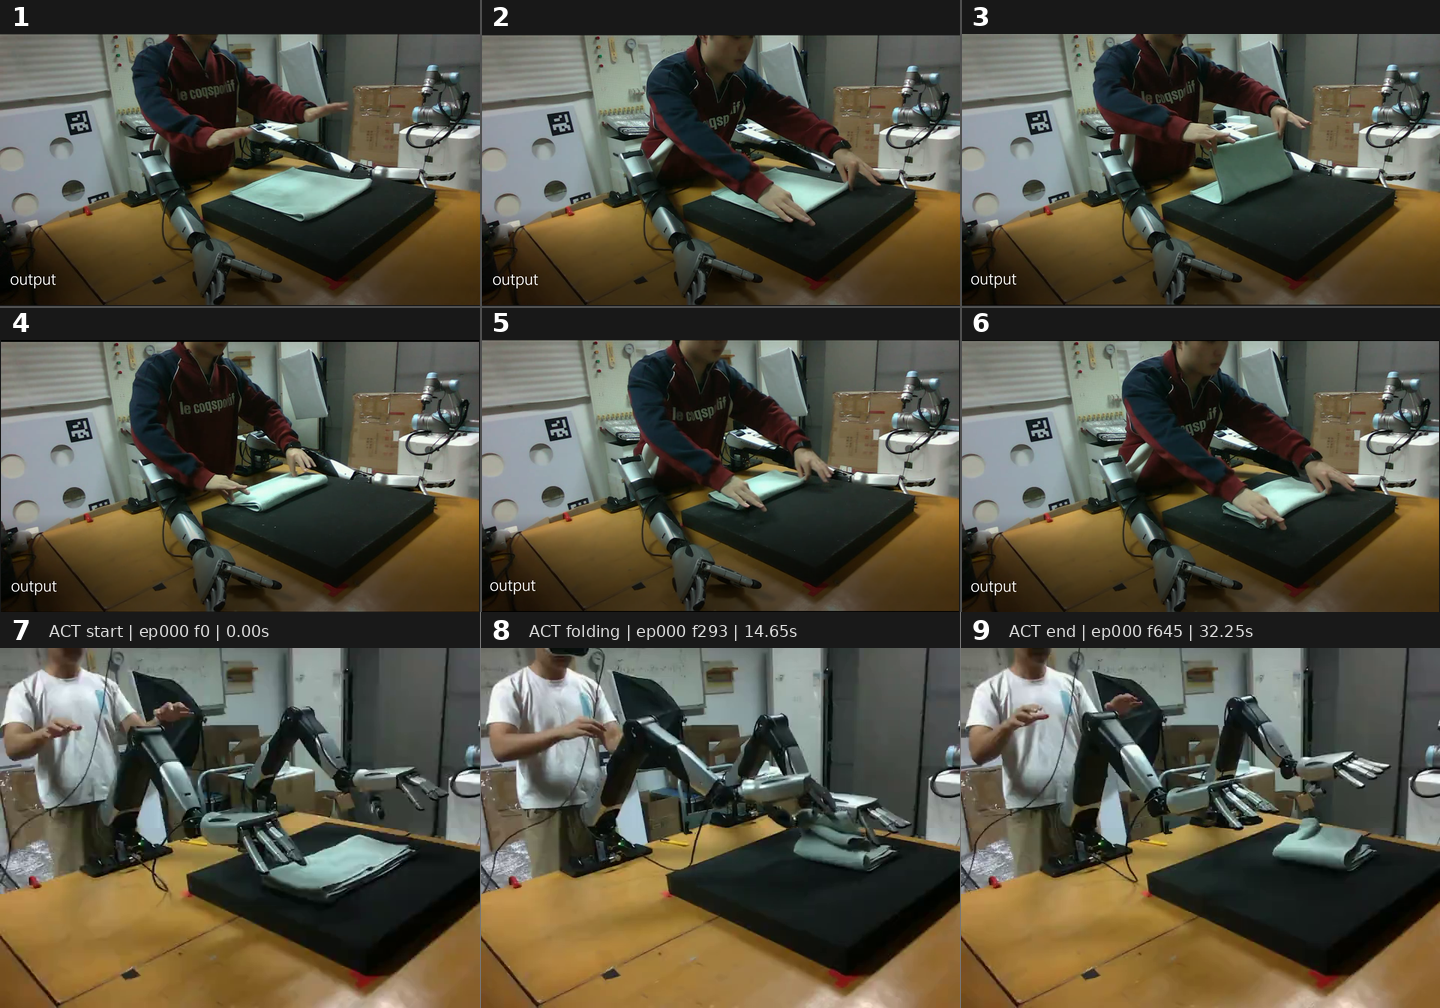
\includegraphics[width=0.92\textwidth]{../../cloth_agent/task/task_sequence.png}
\caption{双阶段毛巾对折与居中交接规程（图 1 至图 6）及双臂 ACT 策略实机自主完成二次对折的关键帧（图 7 至图 9）}
\label{fig:task-sequence}
\end{figure}

表~\ref{tab:dinov3-ablation} 给出了在二次对折 60 条轨迹数据集、相同动作块超参数（$k=60, n=20$）与 $50,000$ 步训练预算下，标准微调 ResNet18 主干与冻结 DINOv3 ViT-S/16 加状态高斯噪声（$\sigma_s = 0.01$）改进模型的对比结果，其中跨光照测试通过调整室内顶灯亮度改变桌面照度后评估动作预测误差与实机二次对折条件成功率。

\begin{table}[htbp]
\centering
\caption{二次对折策略在 50,000 步训练后的视觉主干与状态正则对比评估}
\label{tab:dinov3-ablation}
\footnotesize
\setlength{\tabcolsep}{4pt}
\begin{tabular}{@{}lccc@{}}
  \toprule
  策略模型配置 & 验证集 $L_1$ & 跨光照 $L_1$ & 跨光照二折成功率 \\
  \midrule
  端到端微调 ResNet18 基线 ACT & $0.064$ & $0.118$ & $13 / 18$ ($72.2\%$) \\
  冻结 DINOv3 ViT-S/16（无状态噪声） & $0.061$ & $0.079$ & $15 / 18$ ($83.3\%$) \\
  冻结 DINOv3 ViT-S/16 + 状态噪声（$\sigma_s=0.01$） & $0.058$ & $0.072$ & $17 / 18$ ($94.4\%$) \\
  \bottomrule
\end{tabular}
\end{table}

从表~\ref{tab:dinov3-ablation} 可以看到，端到端微调 ResNet18 主干在同分布验证帧上可取得较低重建误差，但当室内照明亮度发生变化时，归一化动作块 $L_1$ 误差上升至 $0.118$，实机二次对折时偶发提前松指或接近高度偏高。替换为冻结权重的 DINOv3 ViT-S/16 密集补丁特征后，跨光照条件下的动作预测退化明显减小；进一步叠加训练期标准化本体状态高斯噪声正则后，解码器对单步关节反馈自回归外推的依赖减弱，对双层毛巾边缘位置的微小偏移响应更为一致，跨光照条件成功率提升至 $94.4\%$。

在端到端全流程实机评估中，每次试验前将浅绿色矩形毛巾随机平铺于黑色工作垫上，使毛巾中心在桌面 $XY$ 平面内具有 $\pm 12\,\mathrm{cm}$ 范围内的随机位置偏移及 $\pm 25^{\circ}$ 范围内的随机初始偏航角。当系统在不借助人工干预的条件下完成连续两次对折，最终毛巾呈四层叠放状态且整体位于工作垫内时计为成功。表~\ref{tab:e2e-results} 汇总了三种控制方案各自连续执行 20 次实机试验的分阶段与端到端成功率。

\begin{table}[htbp]
\centering
\caption{不同控制方案在随机初始平铺条件下的连续 20 次实机折布结果对比}
\label{tab:e2e-results}
\footnotesize
\setlength{\tabcolsep}{3.5pt}
\begin{tabular}{@{}lccc@{}}
  \toprule
  实机测试方案 & 一折摆正成功率 & 二折条件成功率 & 端到端总成功率 \\
  \midrule
  纯双臂 ACT 串联方案（一折 ACT + 二折 ACT） & $11 / 20$ ($55.0\%$) & $9 / 11$ ($81.8\%$) & $9 / 20$ ($45.0\%$) \\
  代码智能体一折 + 无手型对齐切入二折 ACT & $18 / 20$ ($90.0\%$) & $12 / 18$ ($66.7\%$) & $12 / 20$ ($60.0\%$) \\
  代码智能体一折 + 三步状态对齐 + 二折 ACT（完整系统） & $18 / 20$ ($90.0\%$) & $17 / 18$ ($94.4\%$) & $17 / 20$ ($85.0\%$) \\
  \bottomrule
\end{tabular}
\end{table}

在纯双臂 ACT 串联方案中，当初始毛巾落在示范集中的垫面中央附近时，一折策略可正常完成捏角与翻折；但当初始偏航角超过约 $15^{\circ}$ 或待折边靠近工作垫外侧时，60 条示范轨迹的覆盖密度不足导致预测落点产生 $2\sim 4\,\mathrm{cm}$ 偏差，出现单侧抓空后网络仍继续空手执行翻折动作，使第一阶段成功率停留在 $55.0\%$。

改由视觉代码智能体执行第一阶段后，三维像素反投影与俯视增量偏航控制直接根据实时观测角点解算抓取位姿，消除了大范围位置平移带来的外推误差。在 20 次试验中有 3 次因毛巾角部轻微卷曲导致初次闭合未夹牢，智能体在小幅抬升后的观测轮次中识别出单侧布角未离垫，保持另一侧静止并单独补抓滞留角点，成功恢复其中 2 次，使一次对折与居中摆正成功率达到 $90.0\%$；其余 2 次失败发生在双层翻面平移时下层毛巾因重力滑脱展开。

对比表~\ref{tab:e2e-results} 第二行与第三行消融试验可见，若智能体放布后仅执行机械臂关节回位而省略 \texttt{prepare\_act\_hands} 示范首帧手型对齐，灵巧手中指、无名指与小指仍停留在非示范角度，导致 ACT 策略首个预测动作块在手部槽位与腕部下降轨迹上出现瞬态跳变，接近折边时容易推歪双层毛巾，二次对折条件成功率仅为 $66.7\%$。启用完整的三步起始状态对齐后，交接时刻的视觉画面、14 维双臂关节角与 32 维灵巧手有效槽位均回到训练起始分布内，二次对折在 18 次有效交接中成功 17 次（条件成功率 $94.4\%$），仅 1 次因双层折边未完全对齐而只捏起上层织物，端到端总成功率达到 $85.0\%$。


% -------------------------------------------------------------
\subsection{分工实施情况与工程合作评价}
\label{subsec:team-eval}
% -------------------------------------------------------------

项目开发期间，四个分工模块通过预先约定的坐标转换约定与数据格式并行推进。标定与总线模块输出统一格式的 YAML 标定文件与四通道 SocketCAN 映射，供遥操作模块与代码智能体模块直接复用相同的正逆运动学与虚拟 TCP 几何库；策略训练模块将数据集归一化统计量及示范首帧手型槽位封装为定长二进制管道接口，使硬件控制进程无需耦合深度学习依赖即可在线调用策略。

在中期联调阶段，针对实机测试反映出的单阶段模仿学习在大跨度初始位置下易抓空的问题，团队调整了原本纯神经网络串联的路线，改用代码智能体承担一次对折与居中摆正，并通过三步起始状态对齐衔接双臂 ACT 二次对折策略。


% =============================================================
\section{结论}
\label{sec:conclusion}
% =============================================================

本项目面向两台七自由度机械臂与两套五指灵巧手组成的 46 自由度双臂平台，围绕随机平铺毛巾的连续两次对折任务完成了系统标定、视觉遥操作、动作分块模仿学习与代码生成智能体的集成开发与实机验证。在基础功能上，实现了以共享相机连接左右双臂的九自由度手眼与虚拟 TCP 联合标定（右臂与左臂拟合 RMS 残差分别为 $9.81\,\mathrm{mm}$ 与 $4.86\,\mathrm{mm}$），搭建了集成 Pinocchio 解析雅可比逆运动学（均值耗时 $9.57\,\mathrm{ms}$，较有限差分基线提速 $4.89$ 倍）与对指距离自适应 SLSQP 重定向的 Pico 4 双臂遥操作系统，构建了一次对折与二次对折各 60 条轨迹的多模态数据集，并完成了双臂 ACT 策略的训练与跨环境管道部署。在算法改进与系统耦合上，验证了冻结 DINOv3 ViT-S/16 密集视觉主干配合训练期本体状态高斯噪声正则对提升跨光照稳定性的作用，实现了基于 MCP 与持久 Python 工作进程的双臂折布智能体，并通过三步起始状态对齐串联两个阶段，在连续 20 次随机初始平铺实机测试中取得了 $85.0\%$ 的端到端成功率。

现阶段系统在实际运行中仍受三方面条件制约。第一，全局感知仅依靠单台倾斜顶视安装的 RealSense L515 相机，双臂灵巧手同步伸入垫面中央上方捏布时手掌与前臂会遮挡局部布边，且激光雷达在黑色吸光工作垫与绒面毛巾边缘交界处偶发零深度像素。第二，当前 LinkerHand L20 仅反馈关节位置槽位而未配置指尖触觉或力传感器，单双层织物是否同时夹入指腹只能依靠抬升后的视觉形变间接判断，无法在手指闭合瞬间识别漏夹下层织物。第三，二次对折阶段采用步长 $n=20$（约 $1.0\,\mathrm{s}$）的分段动作队列执行机制，在单个队列窗口内部不更新视觉输入，若双层织物在抬升中途出现轻微滑移，需待当前队列耗尽后才能在下一轮推理中调整轨迹。

后续研究可围绕这三项局限继续改进。感知硬件上，可在左右机械臂腕部加装近距广角相机并融合灵巧手指尖触觉阵列，在手指捏合瞬间直接依据法向与切向接触力判别夹持层数并消除顶视遮挡盲区。策略架构上，可在动作分块主干之上叠加高频轻量级视觉残差修正头，在不牺牲多指闭合连贯性的前提下缩短视觉反馈间隔。任务范围上，可引入织物边缘实例分割与空间点云拓扑提取，将当前面向平铺毛巾的连续对折进一步扩展至从揉乱团状织物自主展平再到多层折叠的完整流程。


% =============================================================
% 参考文献（东南大学毕业论文 GB/T 7714 格式）
% =============================================================
\newpage
\phantomsection
\addcontentsline{toc}{section}{参考文献}
\bibliographystyle{gbt7714-numeric}
\bibliography{refs}

% =============================================================
% 致谢
% =============================================================
\vspace{1.5em}
\phantomsection
\section*{致\quad 谢}
\addcontentsline{toc}{section}{致谢}

感谢《智能机器人系统综合设计》课程授课教师~\todo{指导教师姓名}~老师在课题方案确定、双臂标定设计与阶段检查中给予的指导与修改意见。感谢东南大学相关机器人实验室提供双臂 AgileX Nero 机械臂、LinkerHand L20 灵巧手、深度相机及计算工作站等实验平台支持，同时感谢实验室同学在 CAN 总线配置与实机安全规范方面提供的协助。最后感谢小组成员在数据采集、算法实现与实机调试各阶段的分工合作。

% =============================================================
% 附录
% =============================================================
\newpage
\appendix
% =============================================================
\section{系统总体设计图}
\label{app:system-diagram}
% =============================================================

图~\ref{fig:appendix-full-topology} 给出了双臂灵巧手自主折布系统的硬件通信总线拓扑、跨环境多进程组织结构以及离线采集与在线双阶段执行的数据流向。

\begin{figure}[htbp]
\centering
\resizebox{\textwidth}{!}{%
\begin{tikzpicture}[
  hwbox/.style={rectangle, draw=black!80, rounded corners=3pt, minimum width=3.1cm,
                minimum height=0.95cm, align=center, font=\footnotesize, fill=gray!12},
  procbox/.style={rectangle, draw=black!75, rounded corners=3pt, minimum width=3.4cm,
                  minimum height=1.05cm, align=center, font=\footnotesize},
  envbox/.style={rectangle, draw=black!50, dashed, rounded corners=5pt, inner sep=8pt},
  bus/.style={-{Stealth[length=2.3mm]}, semithick},
  bidir/.style={<->, >=Stealth, semithick}
]
  % 上层 离线遥操作端与在线智能体端
  \node[procbox, fill=blue!8] (pico) at (-4.8, 4.4) {Pico 4 头显追踪端\\TCP 骨骼流 (双手 26 节点)};
  \node[procbox, fill=blue!10] (teleop) at (-4.8, 2.5) {遥操作采集主进程 + 双侧计算子进程\\增量锚定 / 解析 IK / SLSQP 重定向};
  \node[procbox, fill=blue!6] (lerobot) at (-4.8, 0.6) {LeRobot v3.0 数据集存储\\Parquet 状态动作 + H.264 视频};

  \node[procbox, fill=orange!10] (codex) at (0.2, 4.4) {Codex 多模态推理客户端\\视觉分析与代码单元编写};
  \node[procbox, fill=orange!14] (mcp) at (0.2, 2.5) {MCP 协调服务 + 持久工作进程\\准入令牌管理与 \texttt{robo} 轨迹规划};
  \node[procbox, fill=red!10] (hold) at (5.2, 4.4) {独立人工保持终端\\Unix 数据报原位保持};

  % 中层 硬件控制核心与 GPU 推理子进程
  \node[procbox, fill=teal!12, minimum width=4.6cm, minimum height=1.2cm] (ctrl) at (0.2, 0.4) {双臂硬件控制主进程 (\texttt{nero} 环境)\\双侧 $20\,\mathrm{Hz}$ 周期控制器 + 工作区校验};
  \node[procbox, fill=green!12, minimum width=3.8cm, minimum height=1.2cm] (actworker) at (5.5, 0.4) {ACT 常驻推理子进程 (\texttt{act} 环境)\\CVAE/DETR 与冻结 DINOv3 (GPU)};

  % 底层 五路物理硬件接口
  \node[hwbox] (arml) at (-5.4, -2.1) {左臂 AgileX Nero\\(\texttt{can\_arm\_b})};
  \node[hwbox] (handl) at (-1.9, -2.1) {左手 LinkerHand L20\\(\texttt{can\_hand\_b})};
  \node[hwbox] (armr) at (1.7, -2.1) {右臂 AgileX Nero\\(\texttt{can\_arm\_a})};
  \node[hwbox] (handr) at (5.2, -2.1) {右手 LinkerHand L20\\(\texttt{can\_hand\_a})};
  \node[hwbox, fill=cyan!10, minimum width=5.2cm] (cam) at (-0.1, -3.6) {Intel RealSense L515 激光雷达相机\\USB 3.1 对齐 RGB-D 流 ($640\times 480$, $30\,\mathrm{Hz}$)};

  % 连接关系
  \draw[bus] (pico) -- (teleop);
  \draw[bus] (teleop) -- (lerobot);
  \draw[bus, dashed] (lerobot.south) |- ([yshift=0.8cm]actworker.north) -- (actworker.north);

  \draw[bidir] (codex) -- (mcp);
  \draw[bidir] (mcp) -- (ctrl);
  \draw[bus, thick, draw=red!75!black] (hold.south) |- ([yshift=0.25cm]ctrl.east);
  \draw[bidir, thick, draw=green!50!black] (ctrl) -- node[above, font=\scriptsize] {二进制管道} node[below, font=\scriptsize] {状态/图像 $\leftrightarrow$ 46 维动作} (actworker);

  % 硬件连线
  \draw[bidir] (ctrl.south) -- ++(0,-0.45) -| (arml.north);
  \draw[bidir] (ctrl.south) -- ++(0,-0.45) -| (handl.north);
  \draw[bidir] (ctrl.south) -- ++(0,-0.45) -| (armr.north);
  \draw[bidir] (ctrl.south) -- ++(0,-0.45) -| (handr.north);
  \draw[bus] (cam.north) -- ++(0,0.45) -| ([xshift=-0.4cm]ctrl.south);
  \draw[bus, dotted] (teleop.east) -| ([xshift=-1.3cm]ctrl.north);

  % 外框标注
  \begin{scope}[on background layer]
    \node[envbox, fit=(arml)(handl)(armr)(handr)(cam), label={[font=\scriptsize\bfseries]below:物理执行机构、独立四通道 SocketCAN 总线与全局视觉传感层}] {};
  \end{scope}
\end{tikzpicture}%
}
\caption{双臂灵巧手折布系统硬件总线拓扑与跨环境多进程交互设计图}
\label{fig:appendix-full-topology}
\end{figure}


% =============================================================
\section{核心算法与控制器关键代码片段}
\label{app:source-code}
% =============================================================

按照课程报告精简附录代码的要求，以下仅摘录三段核心算法实现片段，完整源码包含于项目代码仓库中。

\subsection{七轴机械臂解析李代数雅可比逆运动学实现}

以下片段取自 \texttt{robot\_control/nero\_ik.py}，对应正文式~\eqref{eq:nero-ik-lsq} 与式~\eqref{eq:nero-ik-jacobian}，实现右不变旋转对数残差及基于 Pinocchio \texttt{Jlog3} 的解析雅可比矩阵计算。

\begin{lstlisting}[caption={七轴逆运动学加权残差与解析雅可比计算片段}]
def residual(candidate):
    actual = self.forward(candidate)
    position = (actual[:3, 3] - target[:3, 3]) / MAX_FK_POSITION_ERROR_M
    rotation = Rotation.from_matrix(target[:3, :3] @ actual[:3, :3].T).as_rotvec()
    rotation /= np.deg2rad(MAX_FK_ROTATION_ERROR_DEG)
    return np.r_[position, rotation,
                 REGULARIZATION_WEIGHT * wrap_angle(candidate - seed)]

def jacobian(candidate):
    actual, frame_jacobian = self._forward_and_jacobian(candidate)
    error_rotation = target[:3, :3] @ actual[:3, :3].T
    rotation_jacobian = -pin.Jlog3(error_rotation) @ frame_jacobian[3:]
    return np.vstack((
        frame_jacobian[:3] / MAX_FK_POSITION_ERROR_M,
        rotation_jacobian / np.deg2rad(MAX_FK_ROTATION_ERROR_DEG),
        REGULARIZATION_WEIGHT * np.eye(7),
    ))
\end{lstlisting}

\subsection{灵巧手对指距离自适应权重与方向解析梯度实现}

以下片段取自优化器模块 \texttt{analytical\_optimizer.py}，对应正文式~\eqref{eq:pinch-alpha} 与式~\eqref{eq:loss-tip}，实现拇指与其余四指的对指激活权重计算及末节指骨单位方向向量的投影雅可比回传。

\begin{lstlisting}[caption={对指自适应激活权重与末节单位向量解析梯度计算片段}]
def _compute_pinch_alpha(self, mediapipe_keypoints: np.ndarray) -> np.ndarray:
    thumb_tip = mediapipe_keypoints[self.MP_TIP_INDICES[0]]
    non_thumb_mp_indices = self.mp_finger_indices[1:]
    finger_tips = np.array([mediapipe_keypoints[self.MP_TIP_INDICES[i]]
                            for i in non_thumb_mp_indices])
    distances = np.linalg.norm(finger_tips - thumb_tip, axis=1) * M_TO_CM
    alphas_nt = np.clip((self.d2 - distances) / (self.d2 - self.d1 + 1e-8),
                        0.0, self.pinch_alpha_max)
    return np.concatenate([[np.max(alphas_nt)], alphas_nt])

# 末节指骨单位方向向量的投影雅可比与梯度累加
for i in range(nf):
    grad_coeff = alphas[i] * self.w_dir * huber_grad_dir[i]
    u = robot_tip_dirs[i]
    n = robot_tip_dir_norm[i, 0]
    J_norm = (np.eye(3) - np.outer(u, u)) / (n + 1e-8)
    J_diff = J_task[i] - J_link4[i]
    total_grad += grad_coeff * (diff_normed_dir[i] @ J_norm @ J_diff)
\end{lstlisting}

\subsection{冻结 DINOv3 密集特征池化与训练期状态噪声注入实现}

以下片段取自策略训练模块 \texttt{train\_act\_dinov3.py}，对应正文式~\eqref{eq:dinov3-proj} 与式~\eqref{eq:state-noise}，实现无梯度提取 DINOv3 局部补丁特征、二维空间平均池化以及训练期标准化本体状态高斯噪声注入。

\begin{lstlisting}[caption={冻结 DINOv3 视觉特征提取与标准化状态噪声注入片段}]
class FrozenDINOv3(nn.Module):
    def __init__(self, backbone: nn.Module, pool_stride: int = 2):
        super().__init__()
        self.encoder = backbone.requires_grad_(False).eval()
        self.pool_stride = pool_stride

    def forward(self, images: torch.Tensor) -> dict[str, torch.Tensor]:
        h, w = images.shape[-2:]
        p = self.encoder.patch_size
        with torch.no_grad():
            tokens = self.encoder.forward_features(images)["x_norm_patchtokens"]
            feat = tokens.transpose(1, 2).reshape(images.shape[0], -1, h // p, w // p)
            if self.pool_stride > 1:
                feat = F.avg_pool2d(feat, self.pool_stride)
        return {"feature_map": feat}

def forward(self, batch):
    if self.training and self.config.state_noise_std > 0:
        batch = dict(batch)
        state = batch["observation.state"]
        batch["observation.state"] = state + torch.randn_like(state) * self.config.state_noise_std
    return super().forward(batch)
\end{lstlisting}


\end{document}
